\subsection{\label{sec:corrections}\desg{g12}-Specific Corrections}
The event reconstruction of a particle track in CLAS starts in region 1 of the DC after the track has gone through the target and start counter. To reconstruct the track back to the event vertex, additional energy loss from the target and start counter are included. The standard CLAS ELOSS package provides the required functionality as detailed in \begin{v2}Ref.~\cite{clas.note.eloss}.\end{v2} ELOSS corrects for the energy lost as charged tracks go from the event vertex through the beam pipe, target, and start counter using the Bethe-Bloch equation \cite{pdg} to relate the material characteristics and path length to energy loss. These corrections are standard. In addition, g12 specific corrections have also been derived, including momentum correction and run-dependent beam energy correction. We performed several iteration to obtain the final corrections to remove the correlations between them.Overall, the impact of momentum corrections have been found to be small, consistent with all previous CLAS results. The beam energy corrections are necessary, after applying the energy loss and momentum correction, to align the masses of all known narrow states with the PDG values. With the final g12 correction procedures, these goals have been achieved. The details of these procedures are explained below:

\subsubsection{\label{sec:corrections.pcor}Final-State Particle Momentum Corrections}


The momenta of the tracks as measured by the Drift-Chamber (\texttt{DC}) have a systematic shift within each sector as a function of azimuthal-angle $\phi$ of one of the tracks. This can be seen in the ``transverse momentum balance'' plots shown in Fig.~\ref{fig:pbal.before}. The transverse momentum balance for a given particle is defined as the sum of the momentum of the other particles projected onto the line that is perpendicular to the beam having the same $\phi$ angle as the given particle minus its momentum transverse to the beam.

The procedure used is described in the \desg{CLAS} note for the momentum correction of the g9b dataset\cite{clas.note.g9bpcor}, though we choose to show the transverse (to the beam) momentum balance which is slightly more sensitive to this feature. The resulting transverse momentum and missing mass balance are shown in Figs.~\ref{fig:pbal} and \ref{fig:mmbal}.

The final \desg{g12} momentum corrections are in the clas6 trunk:
\begin{verbatim}
svn co https://jlabsvn.jlab.org/svnroot/clas/trunk/pcor/g12pcor/All_Corrections
\end{verbatim}
where line number 32 in the script 
\begin{verbatim}
g12_corrections.hpp
\end{verbatim}
needs to be modified to the local copy directory, i.e.
\begin{verbatim}
    TString correction_dir="YOUR_DIRECTORYAll_Corrections/";
\end{verbatim}

The code to use the momentum corrections should look something like this:
\begin{verbatim}
#include "g12_corrections.hpp"

/// load up momentum correction parameters
  clas::g12::MomentumCorrection pcor;


///begin loop over charged particles
{
    float newp = Pcor.pcor(oldp, phi, geant3_pid);
}
\end{verbatim}

Where geant3 pid is the particle ID (according to geant3) for \π[+], \π[-], p, \K[+] or \K[-]. For electron/positrons \π[-], \π[+] pid is used.

\begin{figure}\begin{center}
\begin{subfigure}{0.4\columnwidth}
    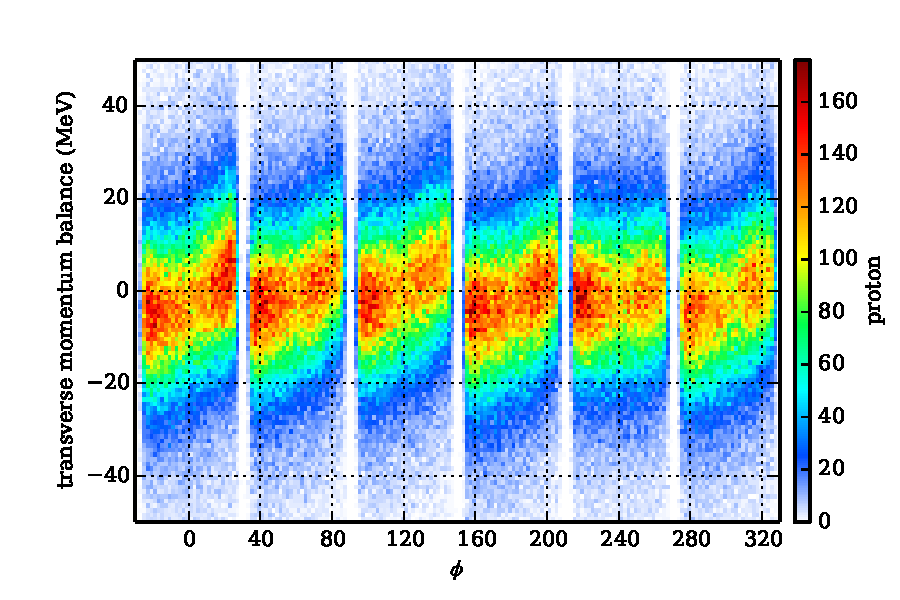
\includegraphics[width=\columnwidth]{figures/pcor/pcor_mptbal_p.pdf}
\end{subfigure}
\begin{subfigure}{0.4\columnwidth}
    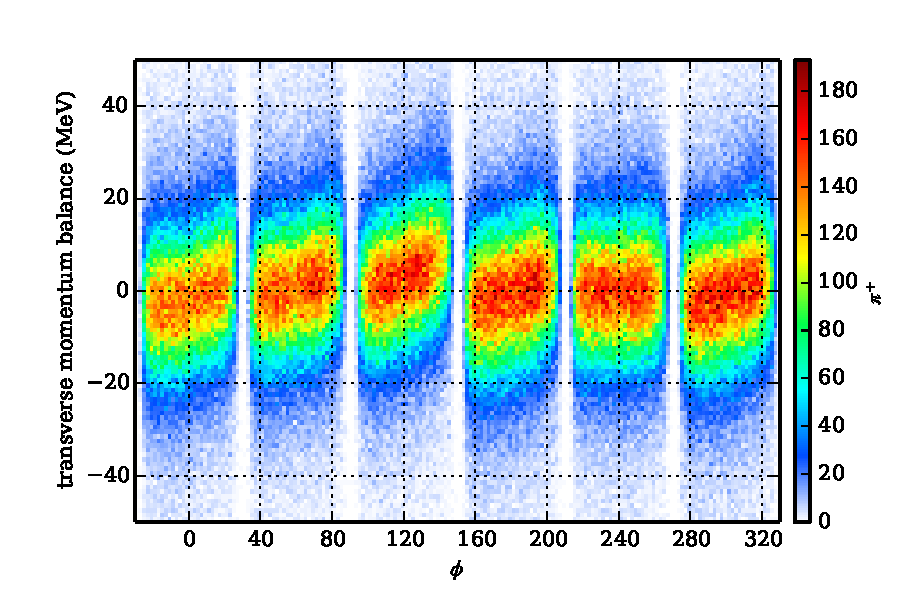
\includegraphics[width=\columnwidth]{figures/pcor/pcor_mptbal_pip.pdf}
\end{subfigure}
\begin{subfigure}{0.4\columnwidth}
    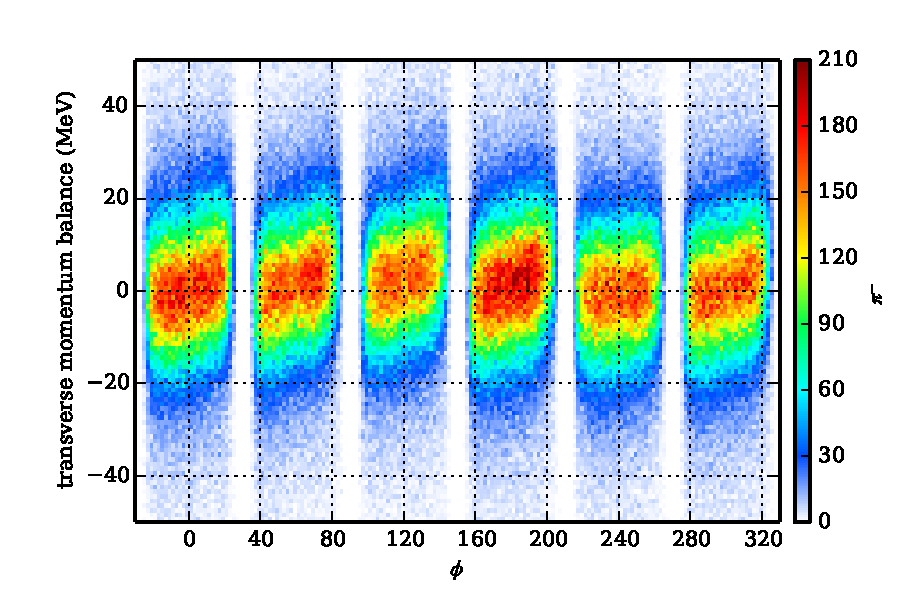
\includegraphics[width=\columnwidth]{figures/pcor/pcor_mptbal_pim.pdf}
\end{subfigure}
\caption[Momentum Balance Before Corrections]{\label{fig:pbal.before}Transverse momentum balance of exclusive p \π[+] \π[-] events as a function of azimuthal angle $\phi$ of each track before momentum corrections for the proton, π$^+$ and π$^-$.}
\end{center}\end{figure}

A simultaneous fit was done by adding a correction to the momenta of each particle for each sector which was linear in $\phi$. The result of the correction is shown in Fig.~\ref{fig:pbal}.

\begin{figure}\begin{center}
\begin{subfigure}{0.4\columnwidth}
    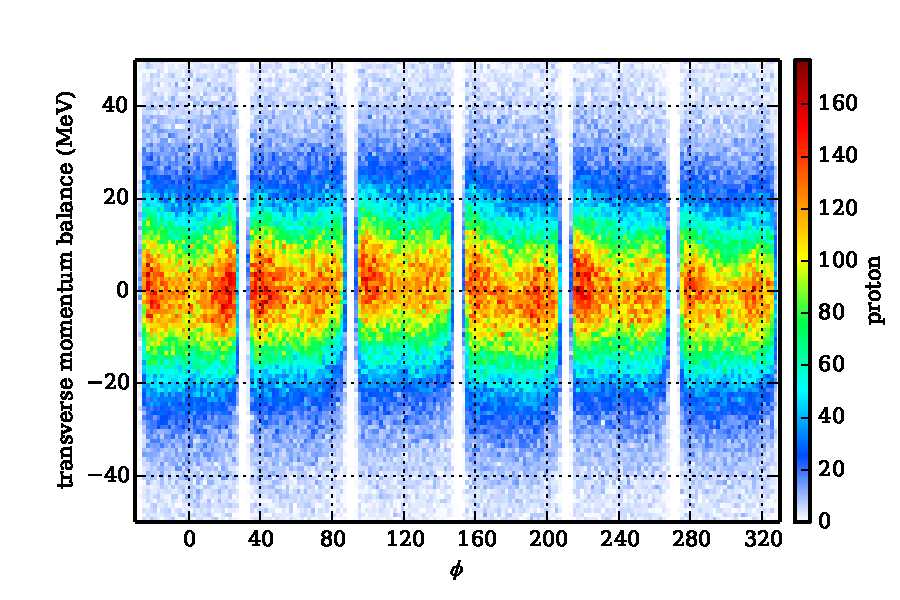
\includegraphics[width=\columnwidth]{figures/pcor/pcor_mptbal_fixed_p.pdf}
\end{subfigure}
\begin{subfigure}{0.4\columnwidth}
    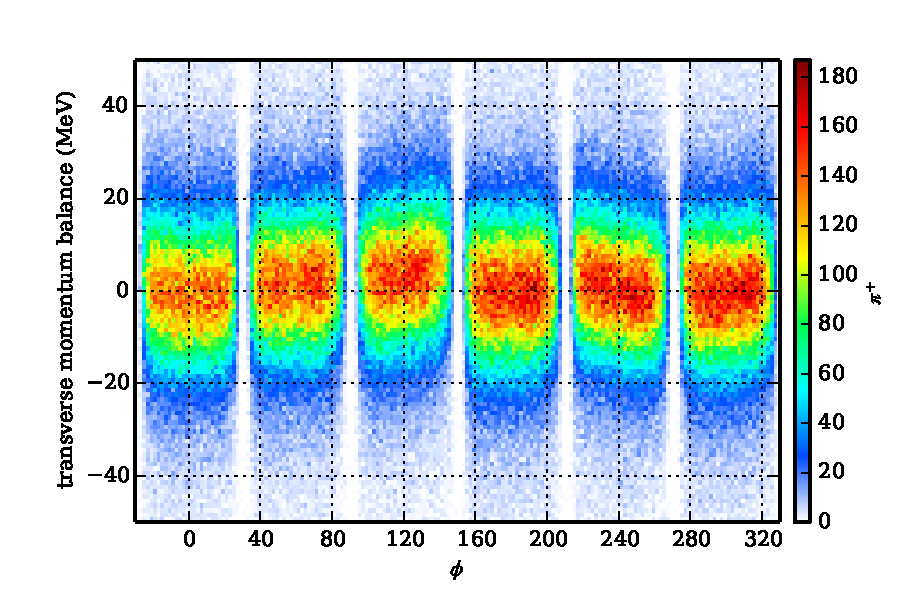
\includegraphics[width=\columnwidth]{figures/pcor/pcor_mptbal_fixed_pip.pdf}
\end{subfigure}
\begin{subfigure}{0.4\columnwidth}
    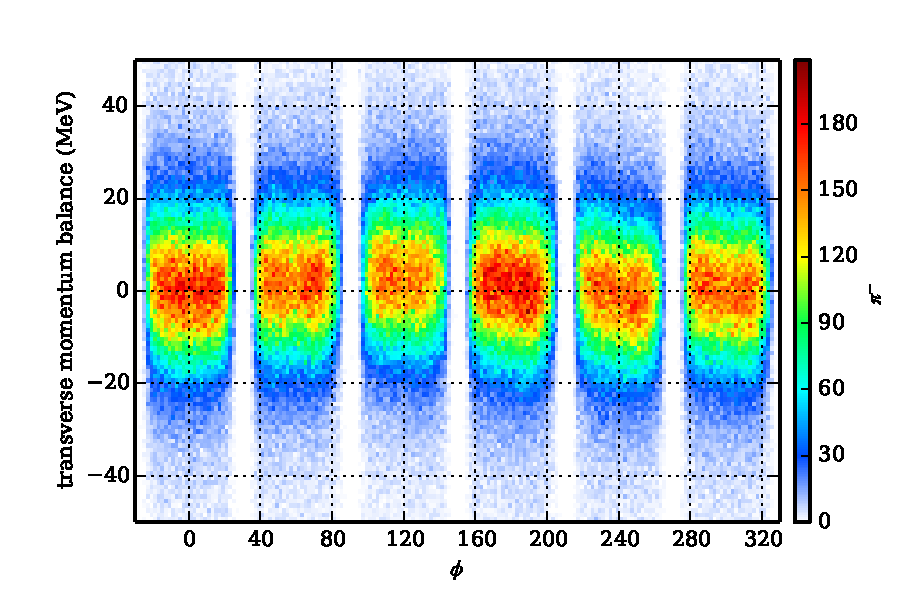
\includegraphics[width=\columnwidth]{figures/pcor/pcor_mptbal_fixed_pim.pdf}
\end{subfigure}
\caption[Momentum Balance Before Corrections]{\label{fig:pbal}Transverse momentum balance of exclusive p \π[+] \π[-] events as a function of azimuthal angle $\phi$ of each track after momentum corrections for the proton, π$^+$ and π$^-$.}
\end{center}\end{figure}

\begin{figure}\begin{center}
\begin{subfigure}{0.4\columnwidth}
    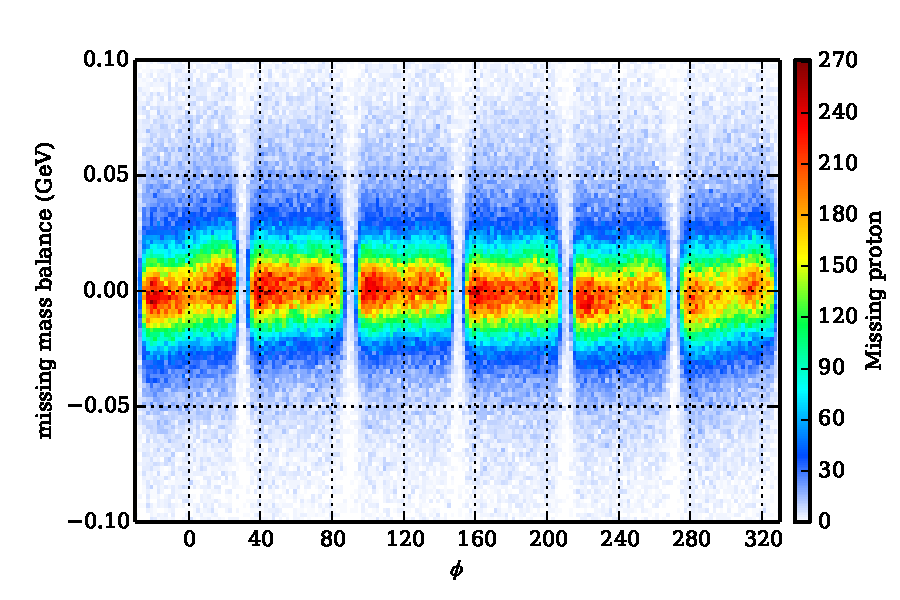
\includegraphics[width=\columnwidth]{figures/pcor/pcor_mpbal.pdf}
\end{subfigure}
\begin{subfigure}{0.4\columnwidth}
    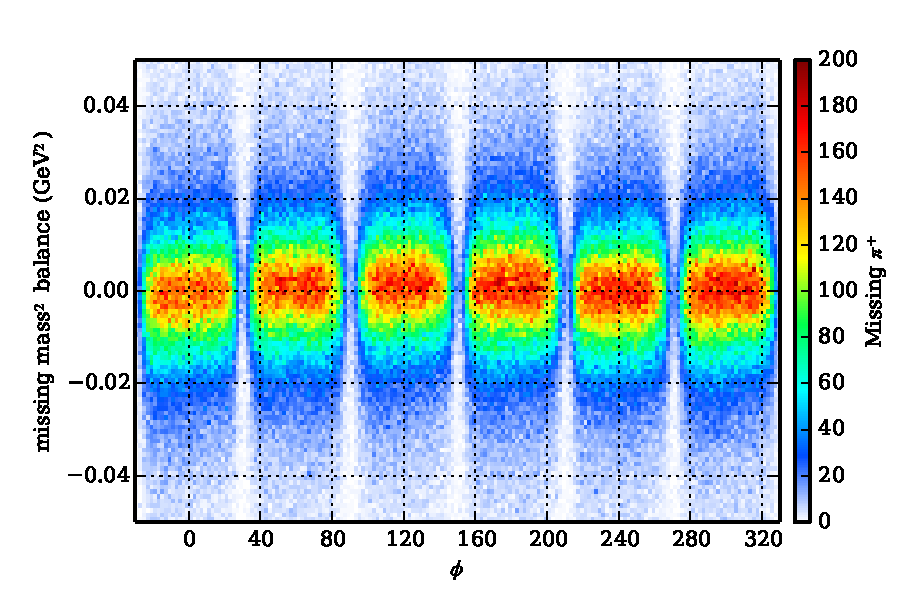
\includegraphics[width=\columnwidth]{figures/pcor/pcor_mpipbal.pdf}
\end{subfigure}
\begin{subfigure}{0.4\columnwidth}
    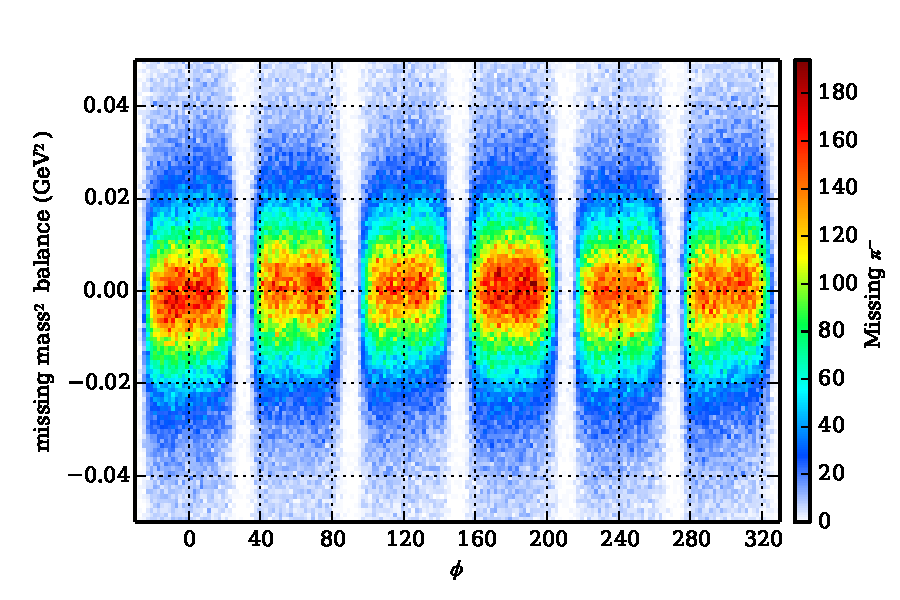
\includegraphics[width=\columnwidth]{figures/pcor/pcor_mpimbal.pdf}
\end{subfigure}
\caption[Momentum Balance Before Corrections]{\label{fig:mmbal}Missing mass (and mass-squared) balance of exclusive p \π[+] \π[-] events as a function of azimuthal angle $\phi$ of each track after momentum corrections for the proton, π$^+$ and π$^-$.}
\end{center}\end{figure}

%\begin{figure}\begin{center}
%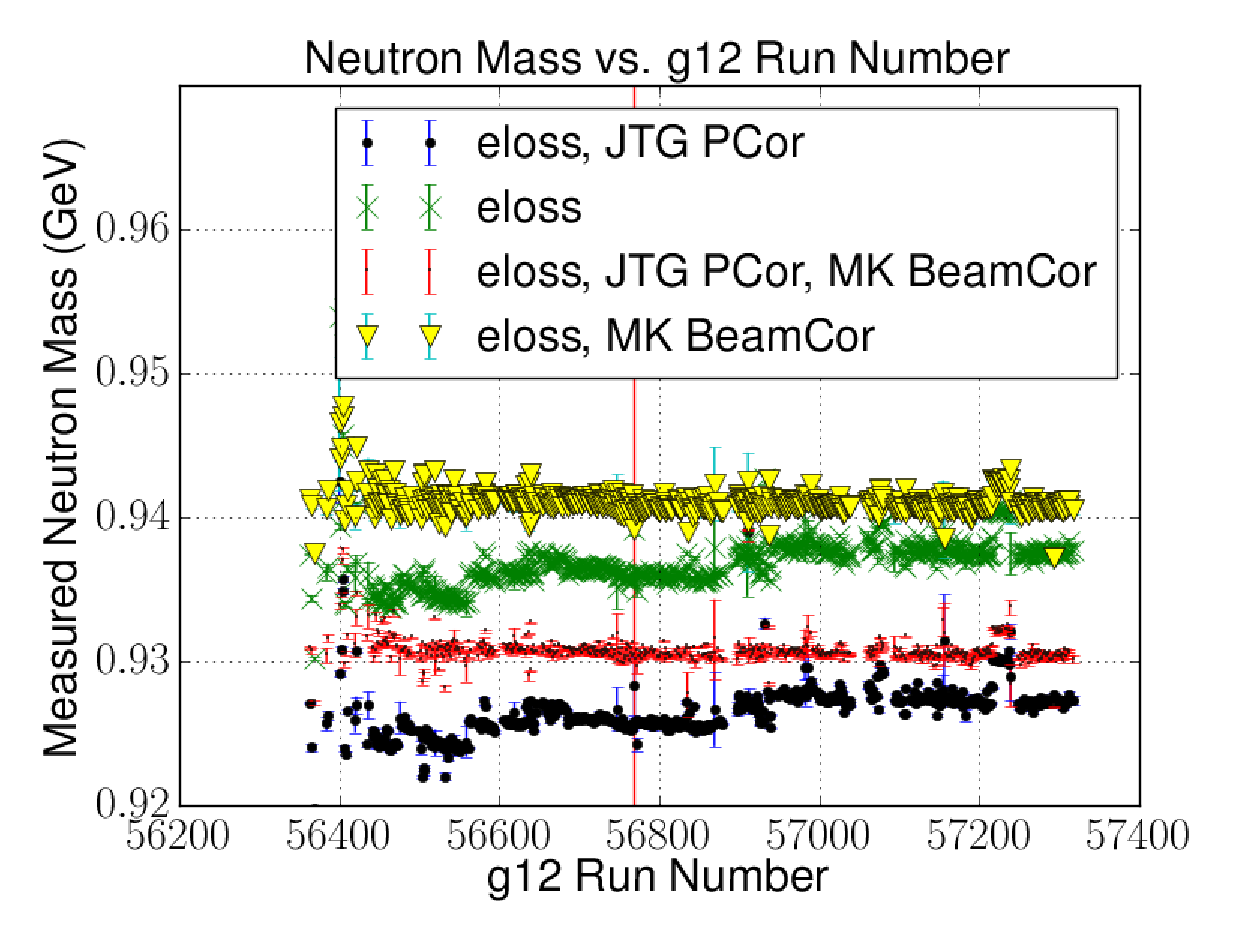
\includegraphics[width=0.6\columnwidth]{figures/corrections/C3pi_allcorr_neutron_rxr.eps}
%\caption[Run by run Mass Balance Before and After Corrections]{\label{fig:mbal_pcor}Neutron mass balance of exclusive n \π[+] \π[+] \π[-] events as a function of run number for before corrections, momentum only, beam only, and after both beam and momentum corrections.}
%\end{center}\end{figure}


\FloatBarrier


\subsubsection{Photon Tagger Calibration and Beam Energy Corrections}

The \desg{g12} experiment had a complicated trigger which presented difficulties that were ironed out as described in this section. The problem was first noticed by \desg{g12} participants at the analysis level in which missing particle masses were systematically low. It was realized while investigating the issue that the low missing particle mass was dependent on the run number and varied in mass as much as 10~MeV. There were also features in the run dependent missing mass that showed a constant low mass (run$<$56550) followed by a jump in mass which remained constant (56500$<$run$<$56920) until another jump in mass which seemed to produce a mass closer the \abbr{PDG} mass (run$>$56920). To analyze and correct for the cause of the problem, two topologies were chosen to isolate the missing particles, proton and neutron. The first topology;
\begin{equation}
    \text{γ p$\rightarrow$π$^+$ π$^-$ p}
    \label{eq:beam.cortopology}
\end{equation}
was chosen to be the correction topology, while the second topology;
\begin{align}
    \text{γ p$\rightarrow$π$^+$ π$^+$ π$^-$ [n]}
    \label{eq:beam.checktopology}
\end{align}
was chosen to verify the corrections obtained from eq.~\ref{eq:beam.cortopology}. The skim consisted of the data for the correction was of one \abbr{CLAS} \abbr{PID} π$^+$, one \abbr{CLAS} \abbr{PID} π$^-$, one \abbr{CLAS} \abbr{PID} proton and nothing else. Exclusive cuts were then placed by requiring the missing energy, $M_E(\text{pπ$^+$π$^-$}) < 0.025$~GeV and the missing mass squared of $M_x^2(\text{pπ$^+$π$^-$}) < 0.015$~GeV$^2$. These cuts assure all events chosen exclude the topology;
\begin{align}
    \text{γ p}\rightarrow\text{p π$^+$ π$^-$ [π$^0$]} \nonumber \,
\end{align}
since the mass squared of π$^0 = 0.0182$~GeV$^2$.

The first step chosen was to verify whether the ``energy-loss'' correction was causing the discrepancy, this can be seen in Figs.~\ref{fig:beamcor.p_mass},~\ref{fig:beamcor.n_mass}. It was concluded that the ``energy-loss'' correction was not the culprit of the problem. From Fig.~\ref{fig:beamcor.p_mass}, two runs were chosen, 56515 and 57130, in which the difference in the missing mass was $\approx$10~MeV. Inspecting the invariant mass, $M$(π$^+$π$^-$), Fig~\ref{fig:beamcor.k_mass}, for runs 56515 and 57130 revealed only a mass deviation of approximately 1.4~MeV, which suggested that the problem with the \desg{g12} data stream is most likely in the photon beam energy.


\begin{figure}\begin{center}
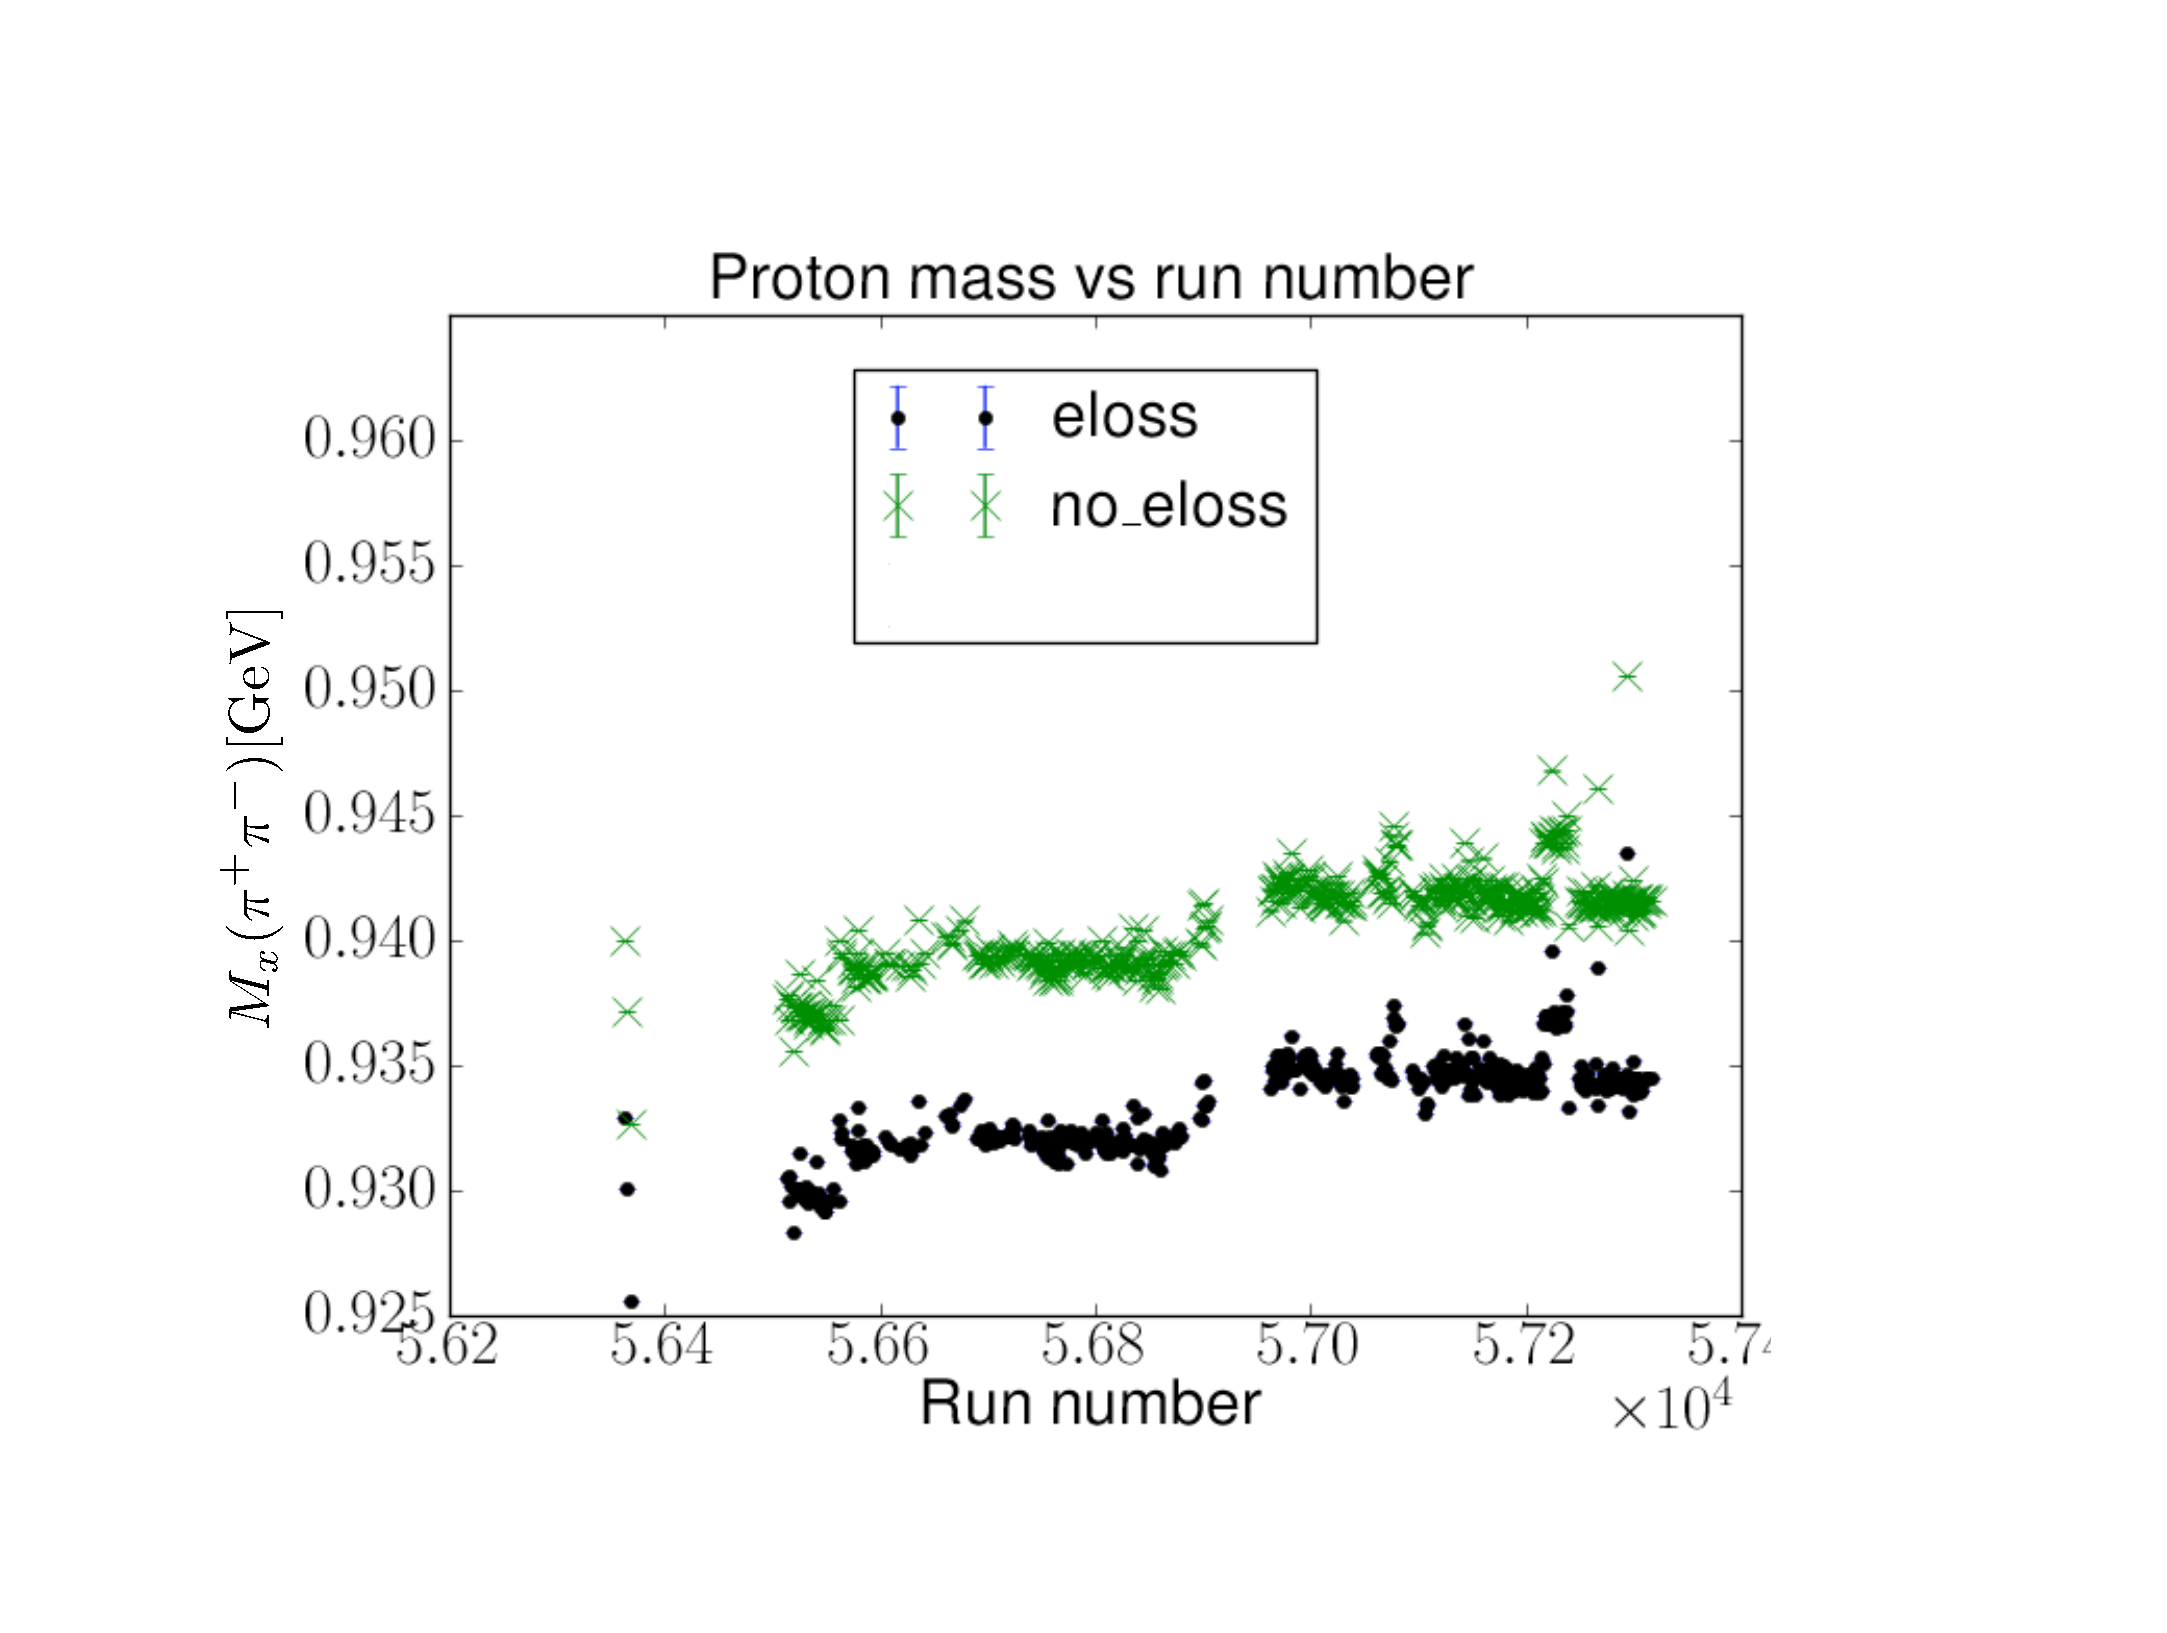
\includegraphics[width=0.6\textwidth]{figures/calib/tag/ecor/P_mass_issue.eps}
\caption[Run Number vs. Proton Mass ]{\label{fig:beamcor.p_mass}Plot of \desg{g12} run number vs. proton mass with and without the ``energy-loss'' applied. See text for details.}
\end{center}\end{figure}

\begin{figure}\begin{center}
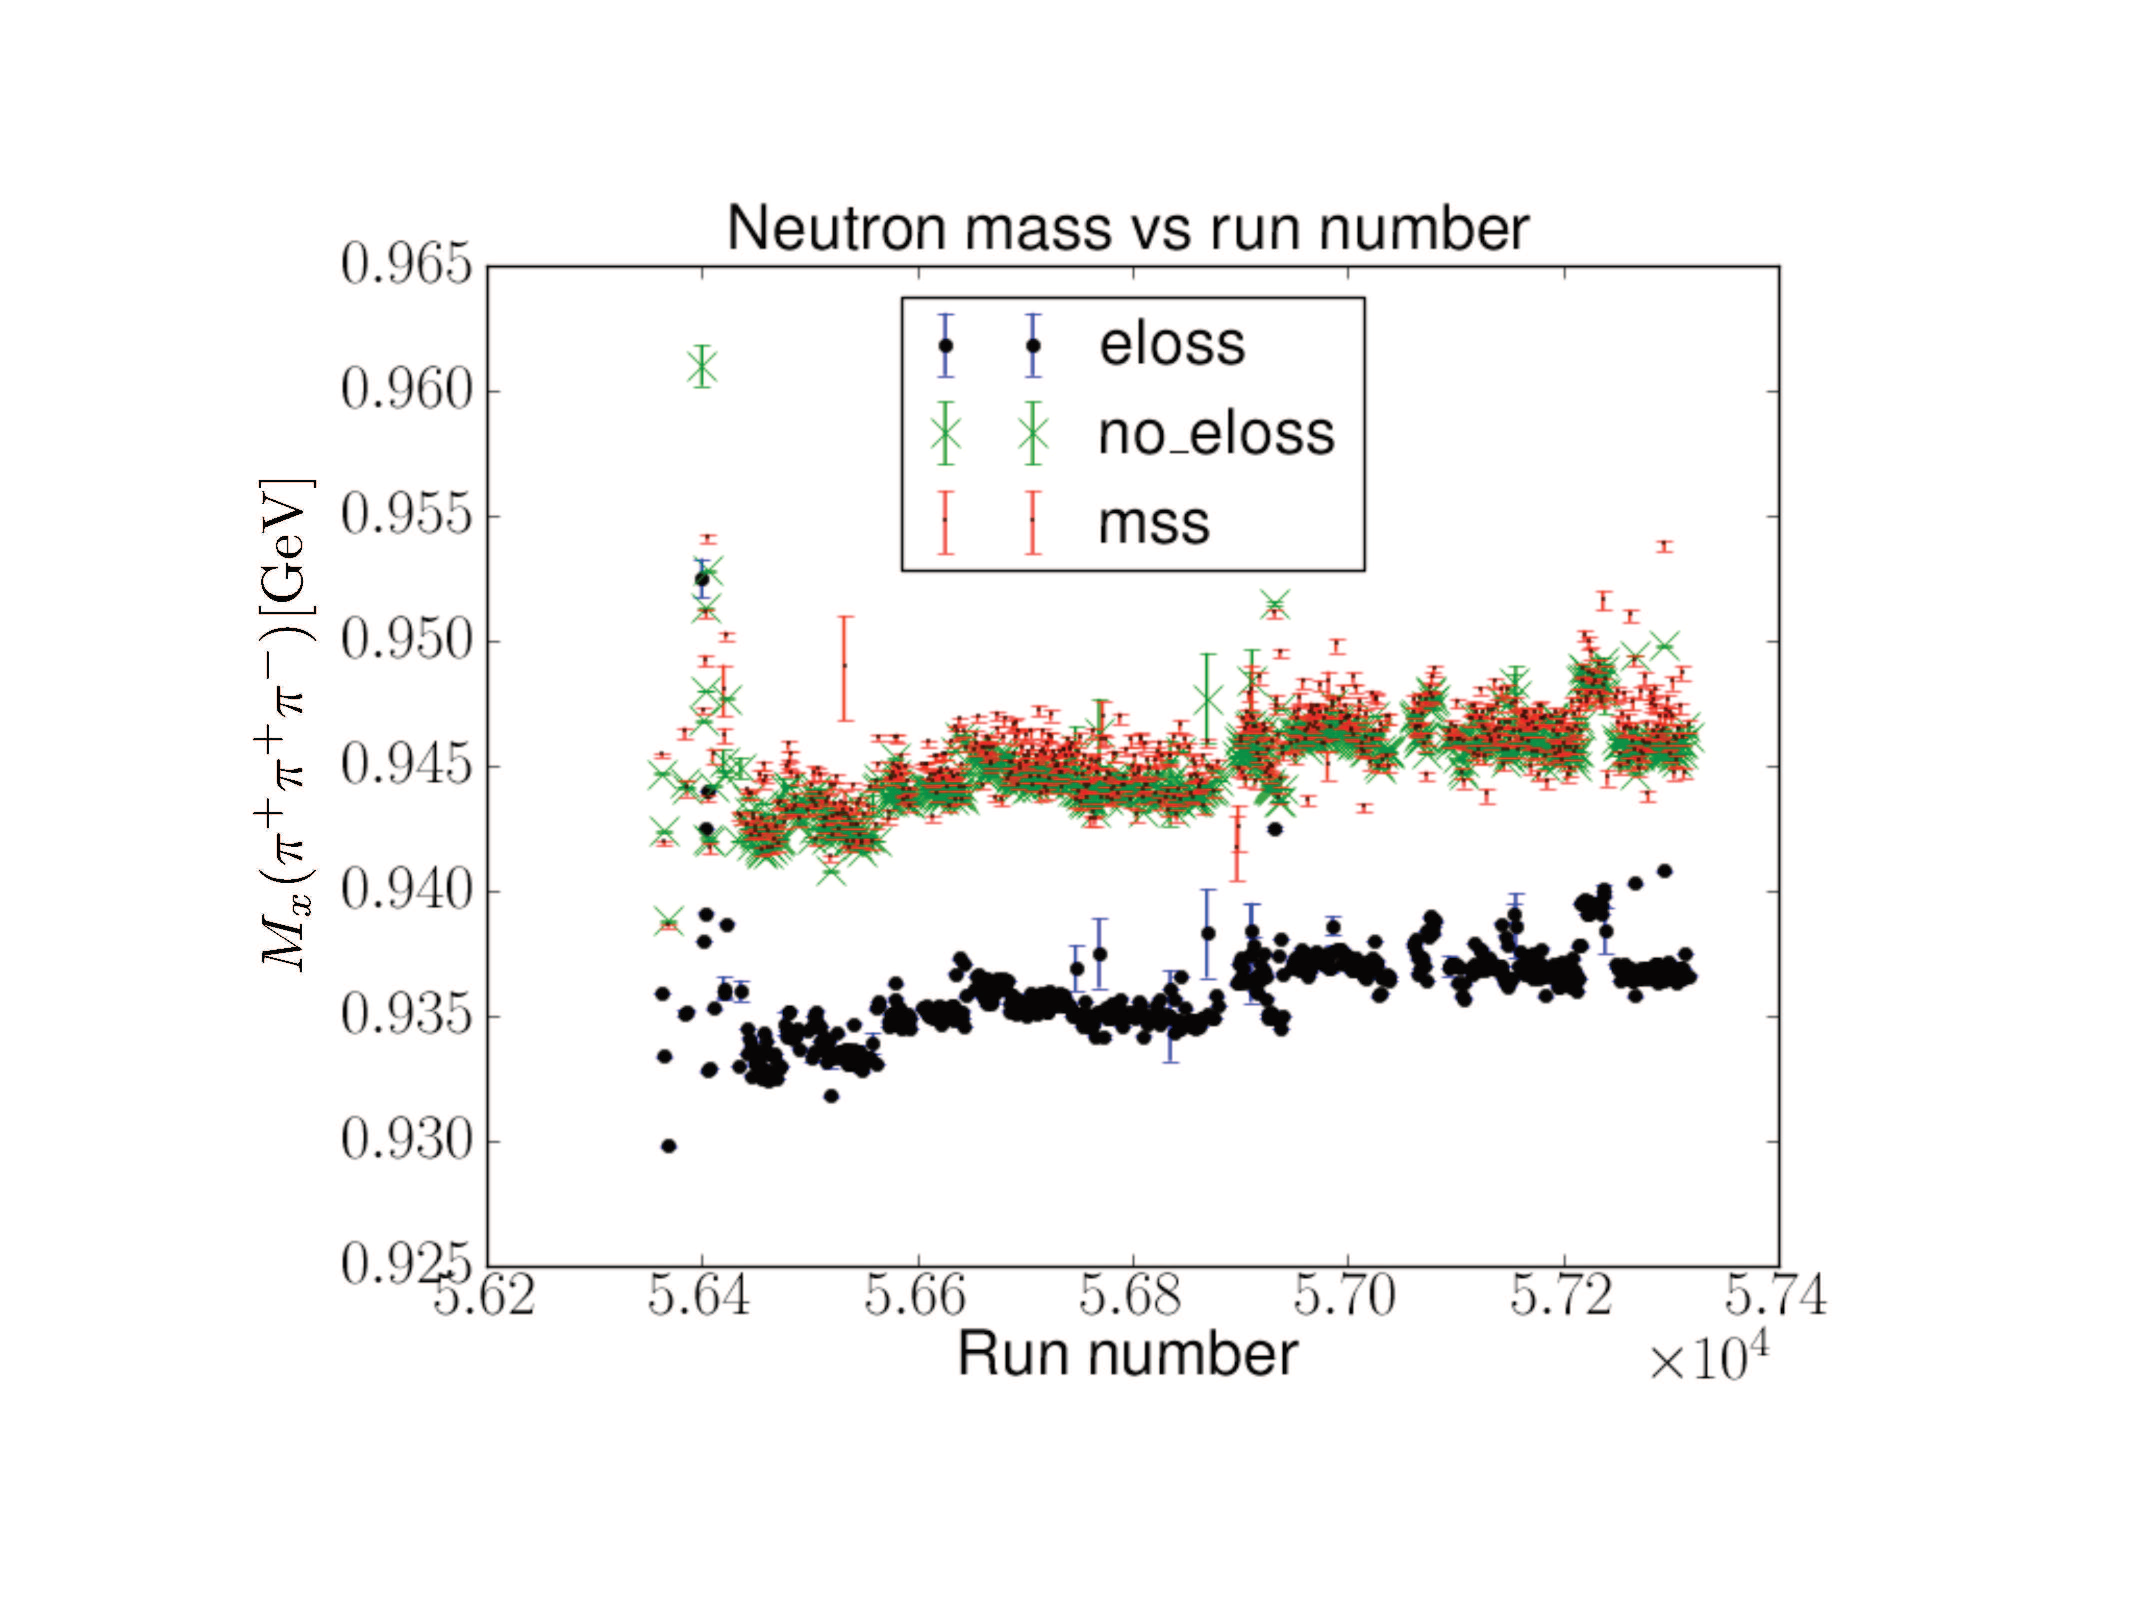
\includegraphics[width=0.6\textwidth]{figures/calib/tag/ecor/N_mass_issue.pdf}
\caption[Run Number vs. Neutron Mass]{\label{fig:beamcor.n_mass}Plot of \desg{g12} run number vs. neutron mass with and without the ``energy-loss'' applied. See text for details. Image Source:~\cite{clas.thesis.bookwalter}}
\end{center}\end{figure}

\begin{figure}\begin{center}
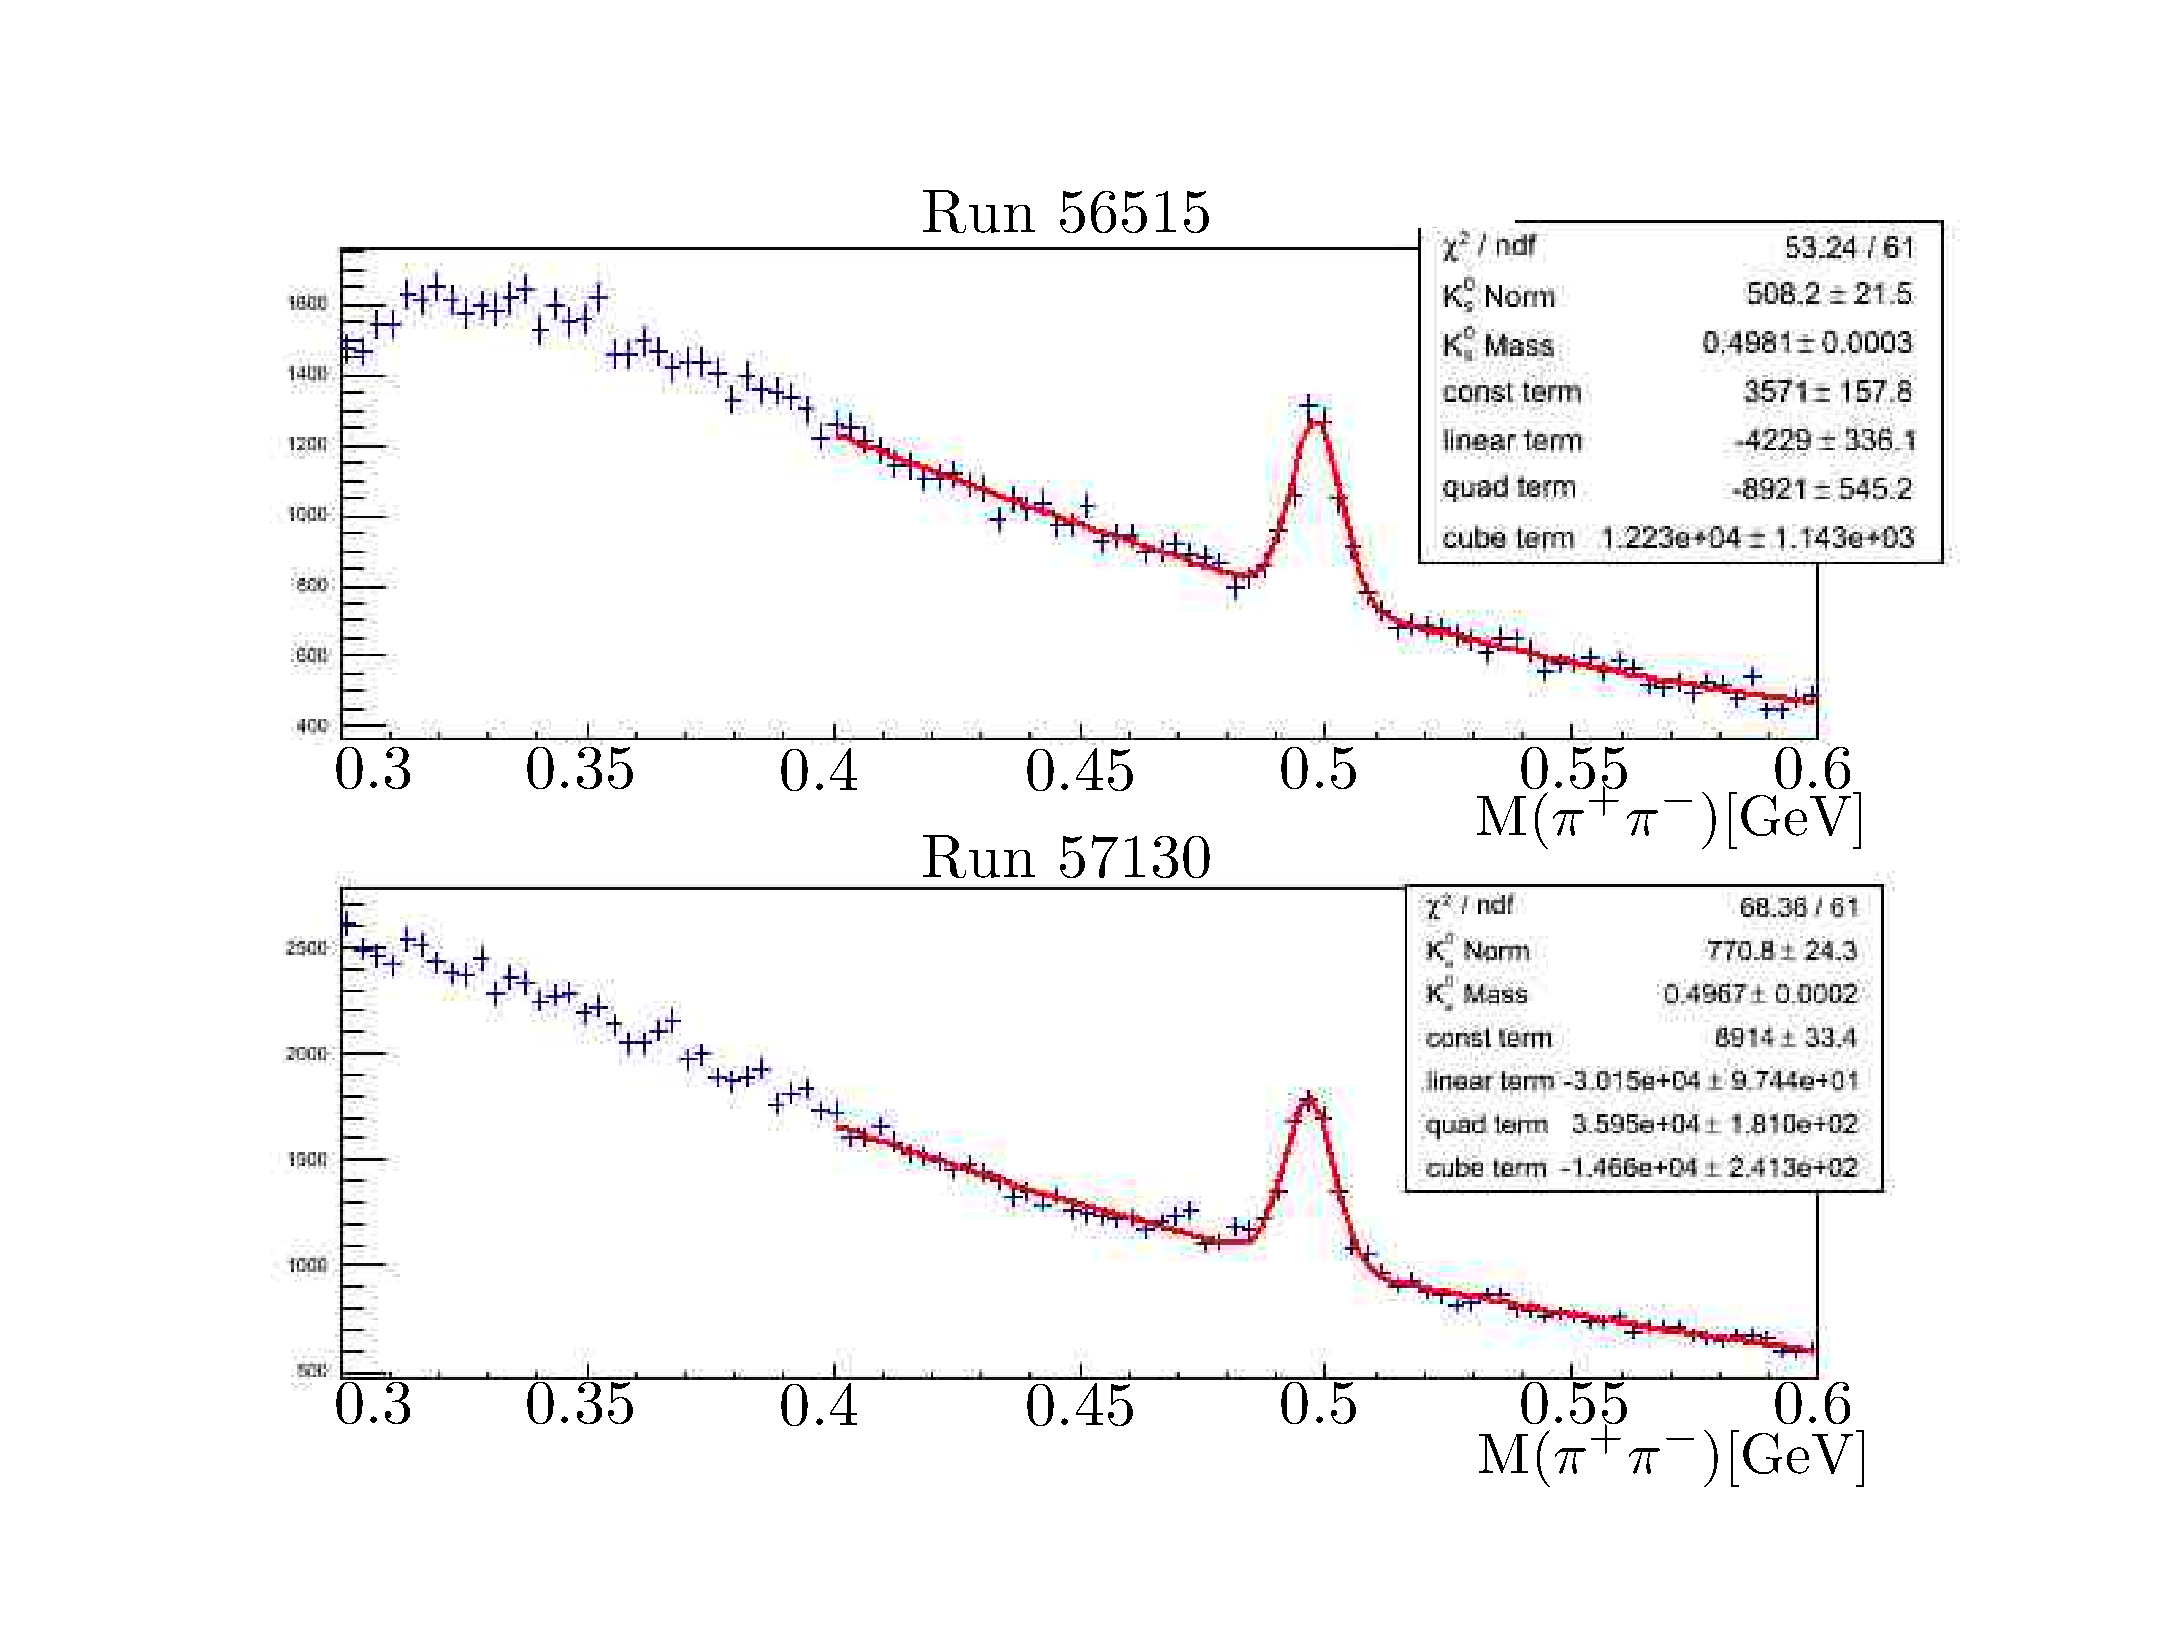
\includegraphics[width=0.75\textwidth]{figures/calib/tag/ecor/Kaon_mass.eps}
\caption[Kaon Mass for Run 56515 and 57130]{\label{fig:beamcor.k_mass}Plot of Kaon mass for runs 56515 and 57130.}
\end{center}\end{figure}

\FloatBarrier

Now that it is known that the photon beam energy is the cause of the issue, it must be known the cause of the photon beam error. Several quantities that the tagger subsystem are subjected to were analyzed, first being the tagger magnet current which, according to the \abbr{EPICS} Fig~\ref{fig:tag.magnet.epics}, remain constant
but showed that around run = 56920 (May 12, 2008) the tagger magnet was shut-off. The tagger magnet shut-off was done because work had to be done in the hall, however after the tagger magnet was turned on, the current was set to its previous setting. A further investigation into the tagger magnet was performed by private communication with the accelerator group chief Arne Freyberger, Fig~\ref{fig:tag.magnet.arne} shows the data the accelerator group had for the tagger magnet which confirms that the tagger magnet current was stable throughout the running of \desg{g12}. The next beam quantity analyzed was the beam \begin{v2}energy\end{v2}\ delivered by \abbr{CEBAF}, again through private communication with the accelerator group chief Arne Freyberger it is shown in Fig.~\ref{fig:beamenergy} that the electron beam \begin{v2}energy\end{v2}\ remained constant throughout the \desg{g12} experiment.
\begin{figure}\begin{center}
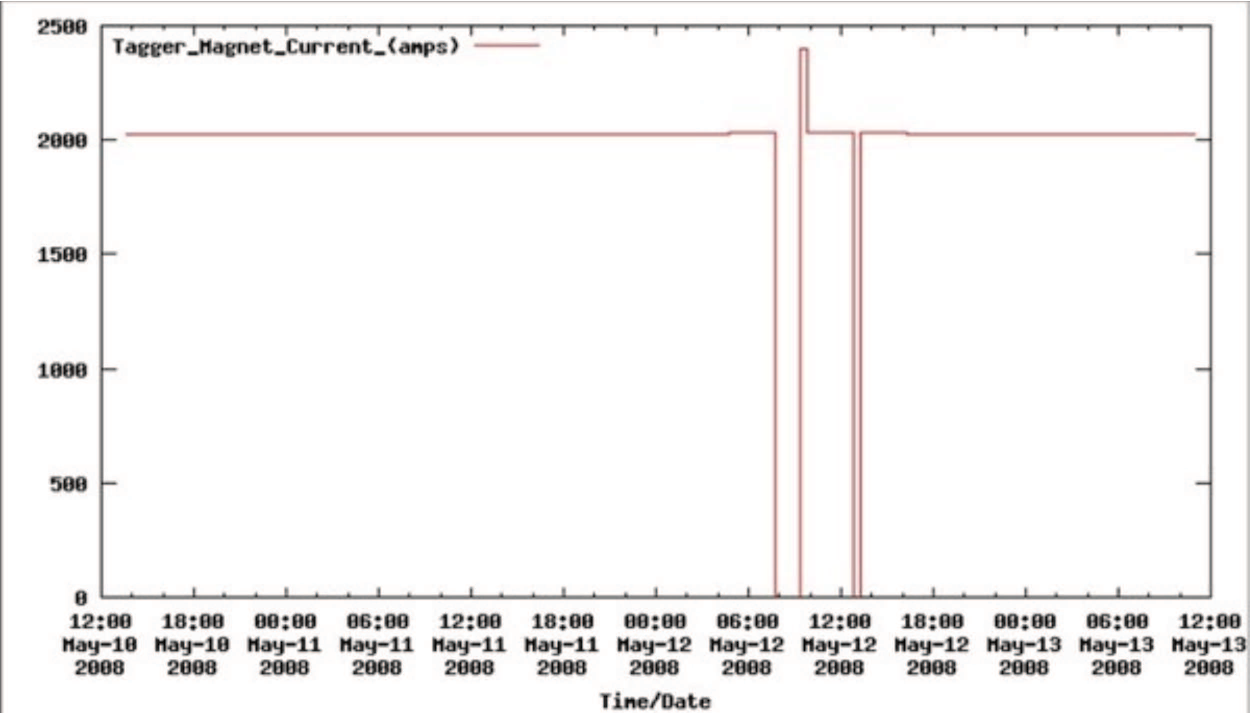
\includegraphics[width=0.6\textwidth]{figures/calib/tag/ecor/600px-Hystersis_smokingGun.pdf}
\caption[Current of Tagger Magnet from \abbr{EPICS}]{\label{fig:tag.magnet.epics}Tagger magnet current according to \abbr{EPICS}}
\end{center}\end{figure}

\begin{figure}\begin{center}
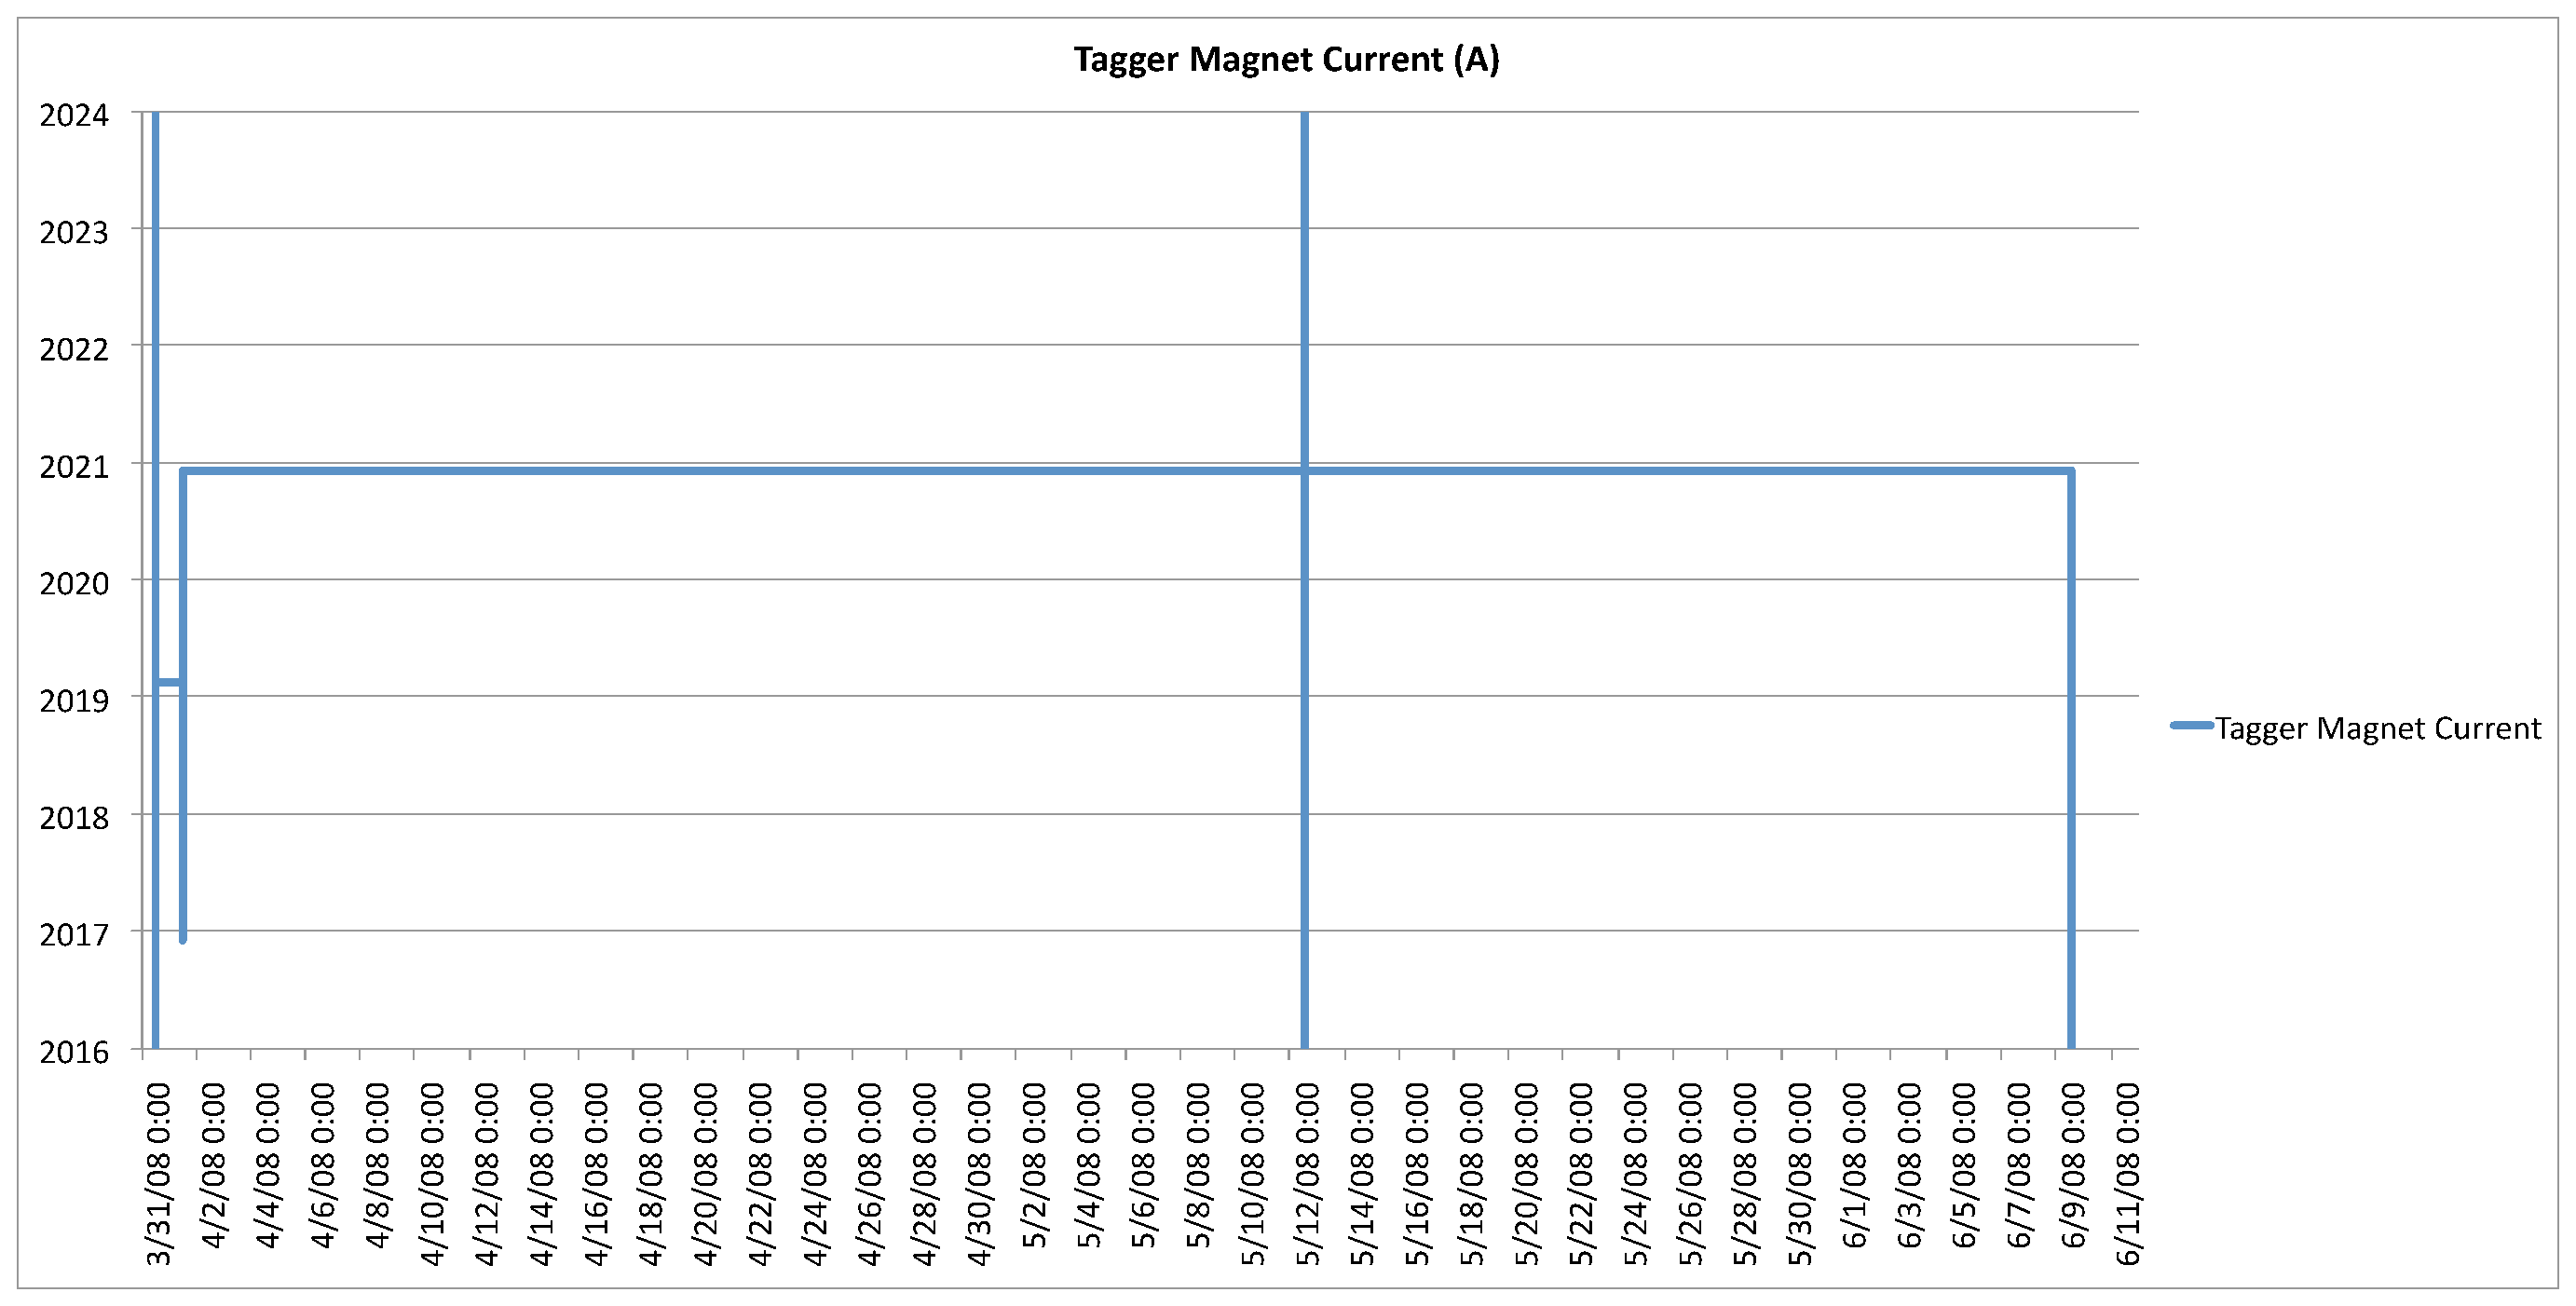
\includegraphics[width=0.6\textwidth]{figures/calib/tag/ecor/tagger_current_arne.eps}
\caption[Current of Tagger Magnet from Accelerator Group]{\label{fig:tag.magnet.arne} Tagger magnet current according to accelerator group}
\end{center}\end{figure}

\begin{figure}\begin{center}
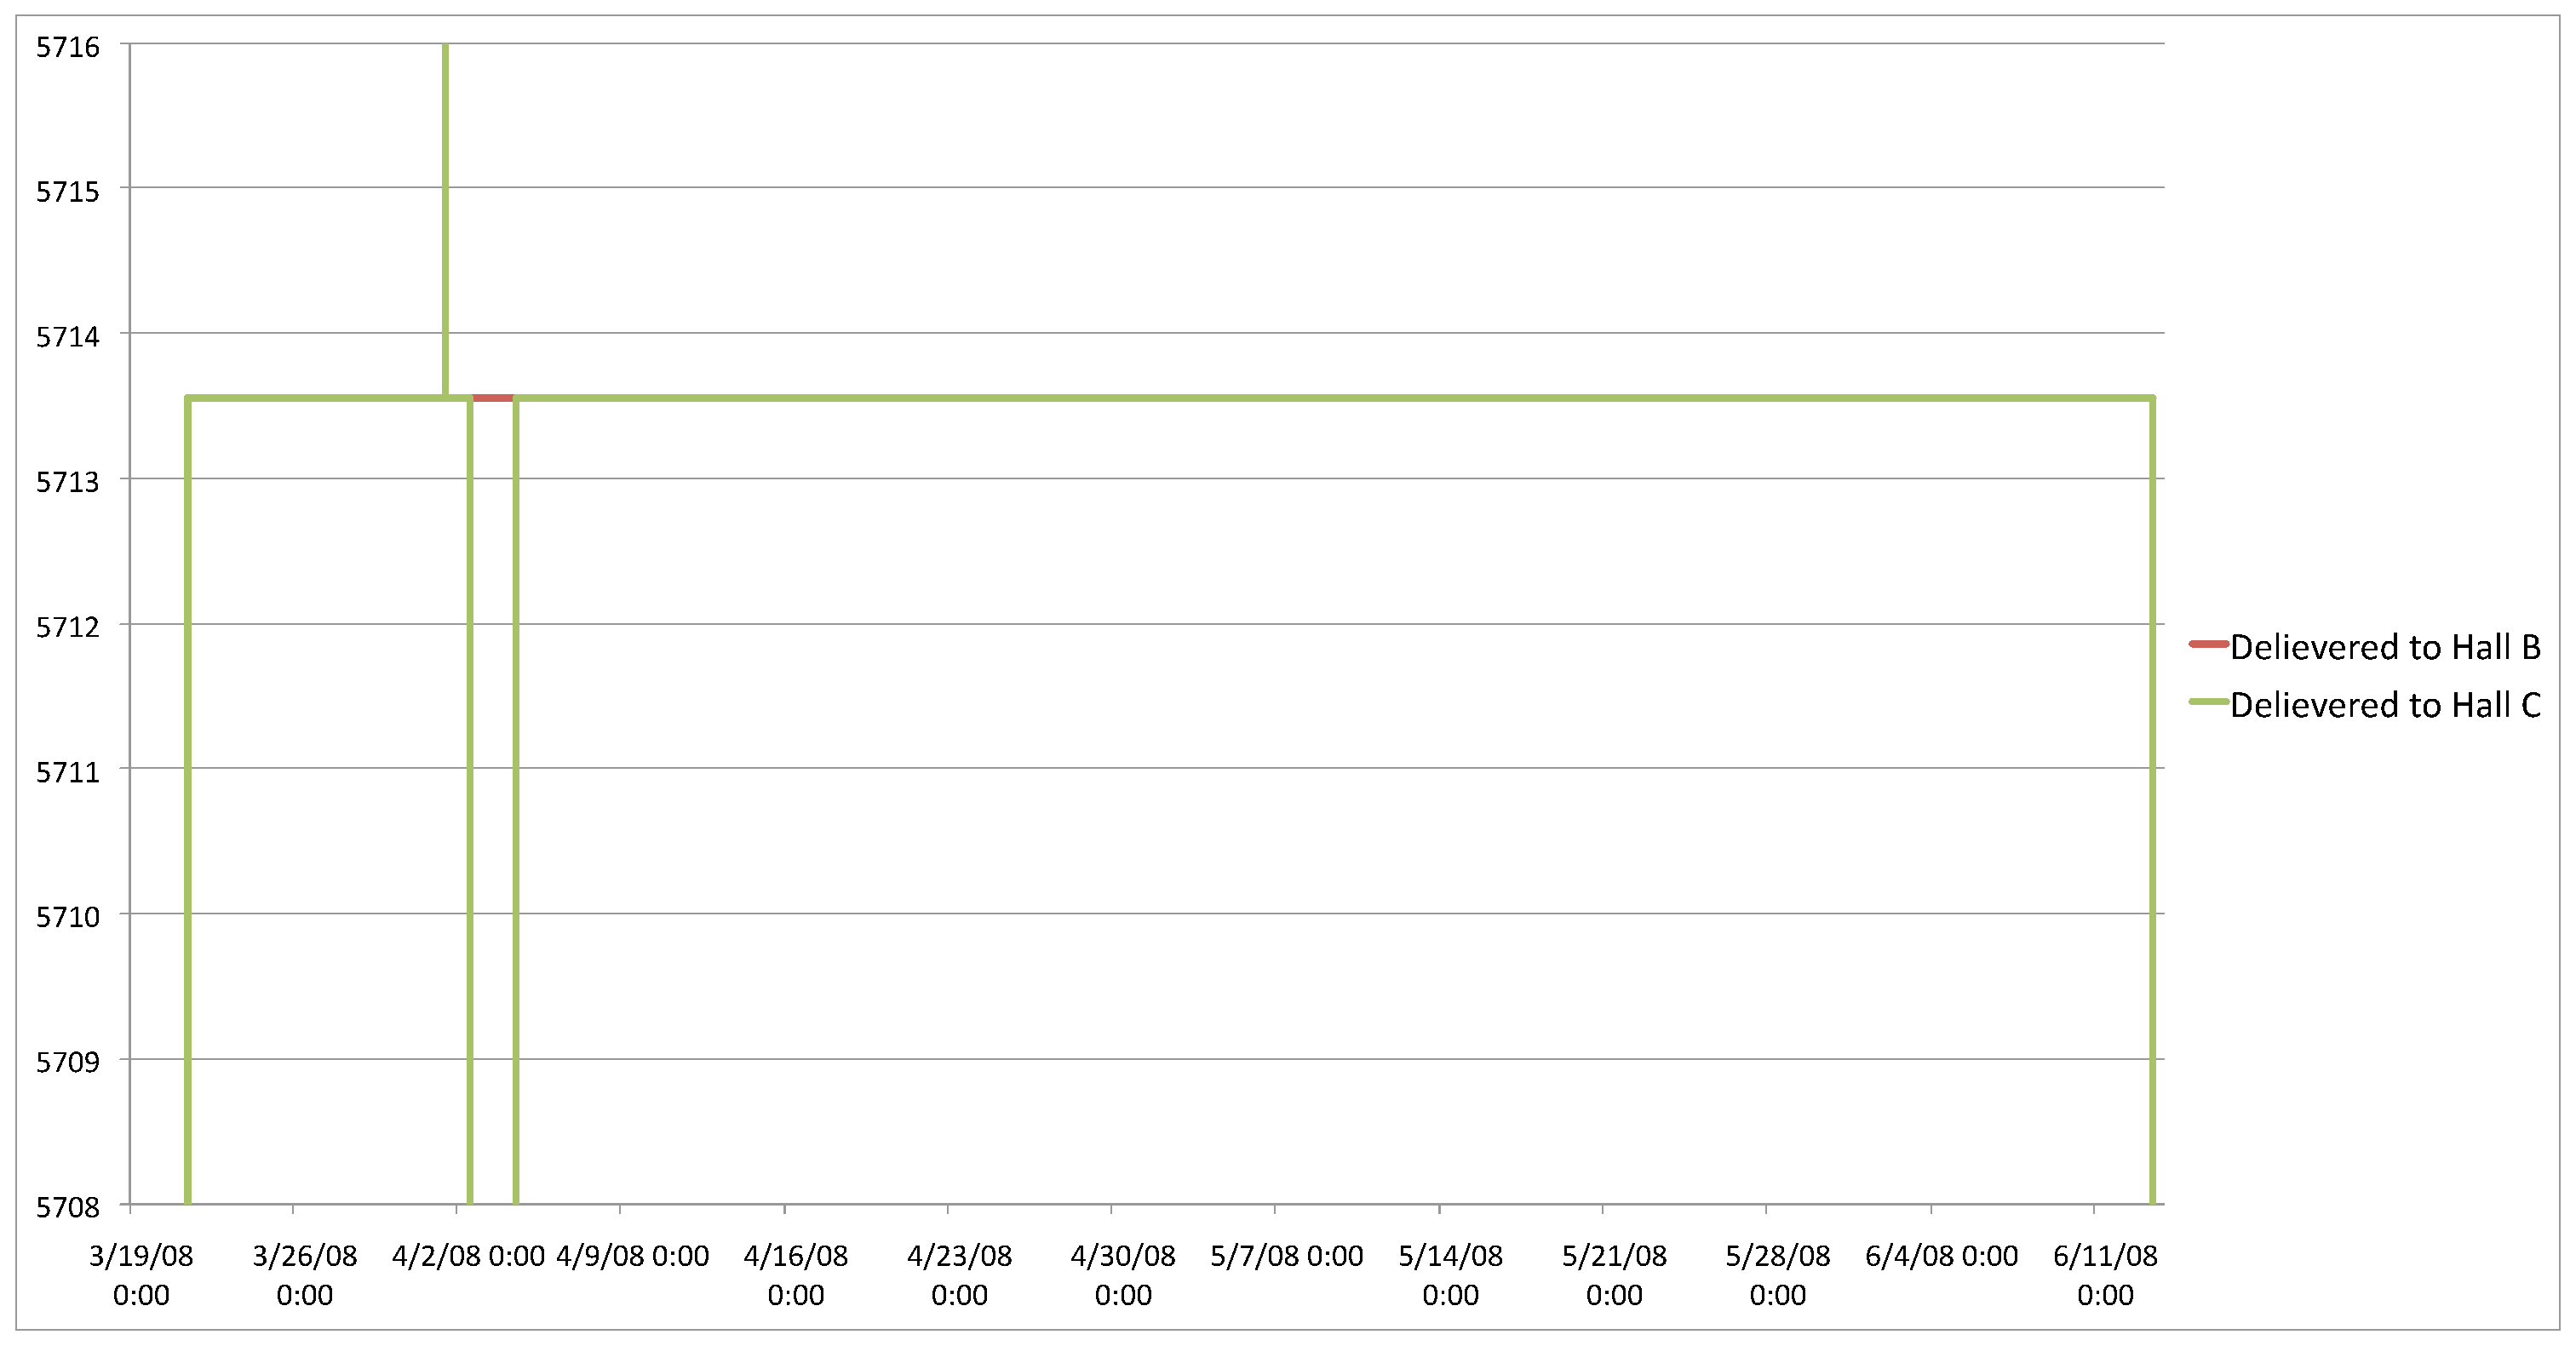
\includegraphics[width=0.6\textwidth]{figures/calib/tag/ecor/beam_currentsII.eps}
\caption[Electron Beam Energy Delivered to hall \desg{b} and hall \desg{c} ]{\label{fig:beamenergy}Electron beam \begin{v2}energy\end{v2}\ delivered to hall \desg{b}(red) and hall \desg{c} (green) according to accelerator group during the time of \desg{g12} running }
\end{center}\end{figure}

The next quantity investigated was the positioning of the tagger dump. Since the radius of curvature a charged particle travels is proportional to the magnetic field, Eq.~\ref{eq:motioninmagII}, this quantity is suitable.
\begin{equation}\label{eq:motioninmagII}
    p = q(v \times B)r
\end{equation}
The y-positioning of the tagger dump jumps on or about May 12, 2008, Fig.~\ref{fig:tagdump}. This would effect how the tagger recorded the scattered electron. A cause for the change in y-positioning can only be due to the magnetic field changing. The phenomena in magnetism that allows for a steady current but a change in magnetic field is known as hysteresis, Fig.~\ref{fig:hyst} illustrates that on the x-axis there is a constant current that is associated with 2 distinct magnetic fields shown on the y-axis of Fig.~\ref{fig:hyst}.
\begin{figure}\begin{center}
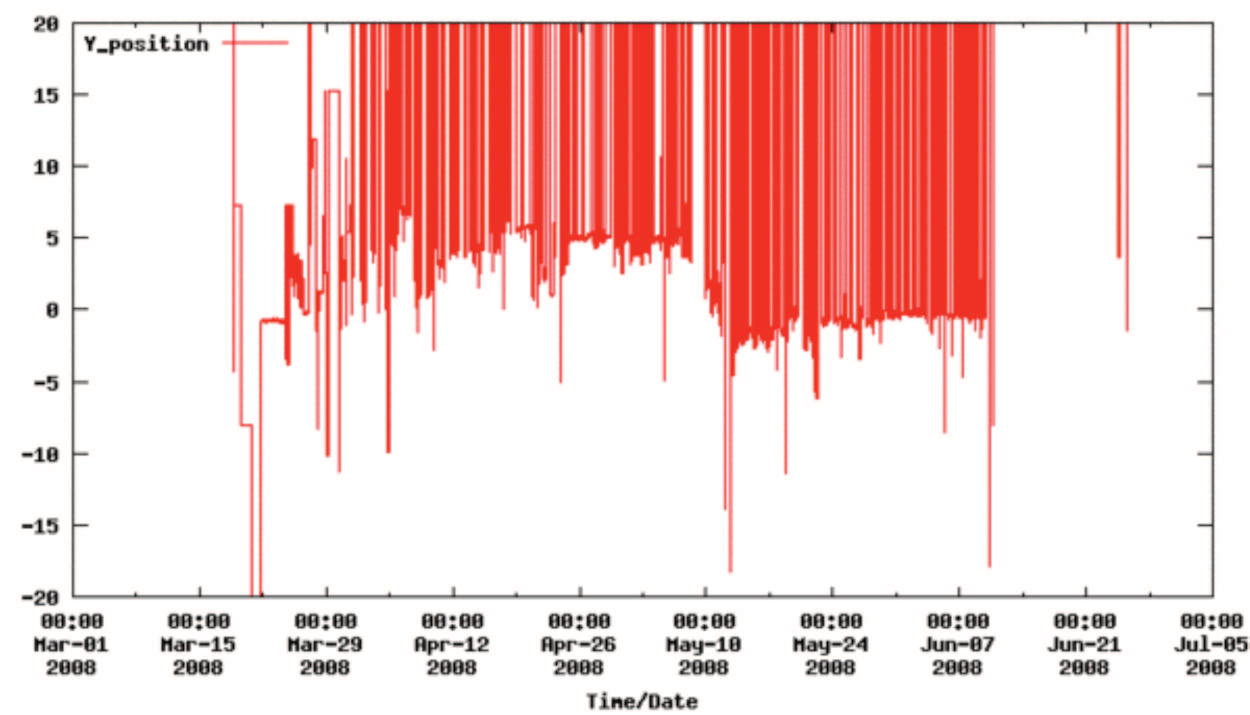
\includegraphics[width=0.6\textwidth]{figures/calib/tag/ecor/600px-Tagger-dump-y.pdf}
\caption[Tagger Dump Y-Positioning]{\label{fig:tagdump}Tagger dump y-positioning according to \abbr{EPICS}}
\end{center}\end{figure}

\begin{figure}\begin{center}
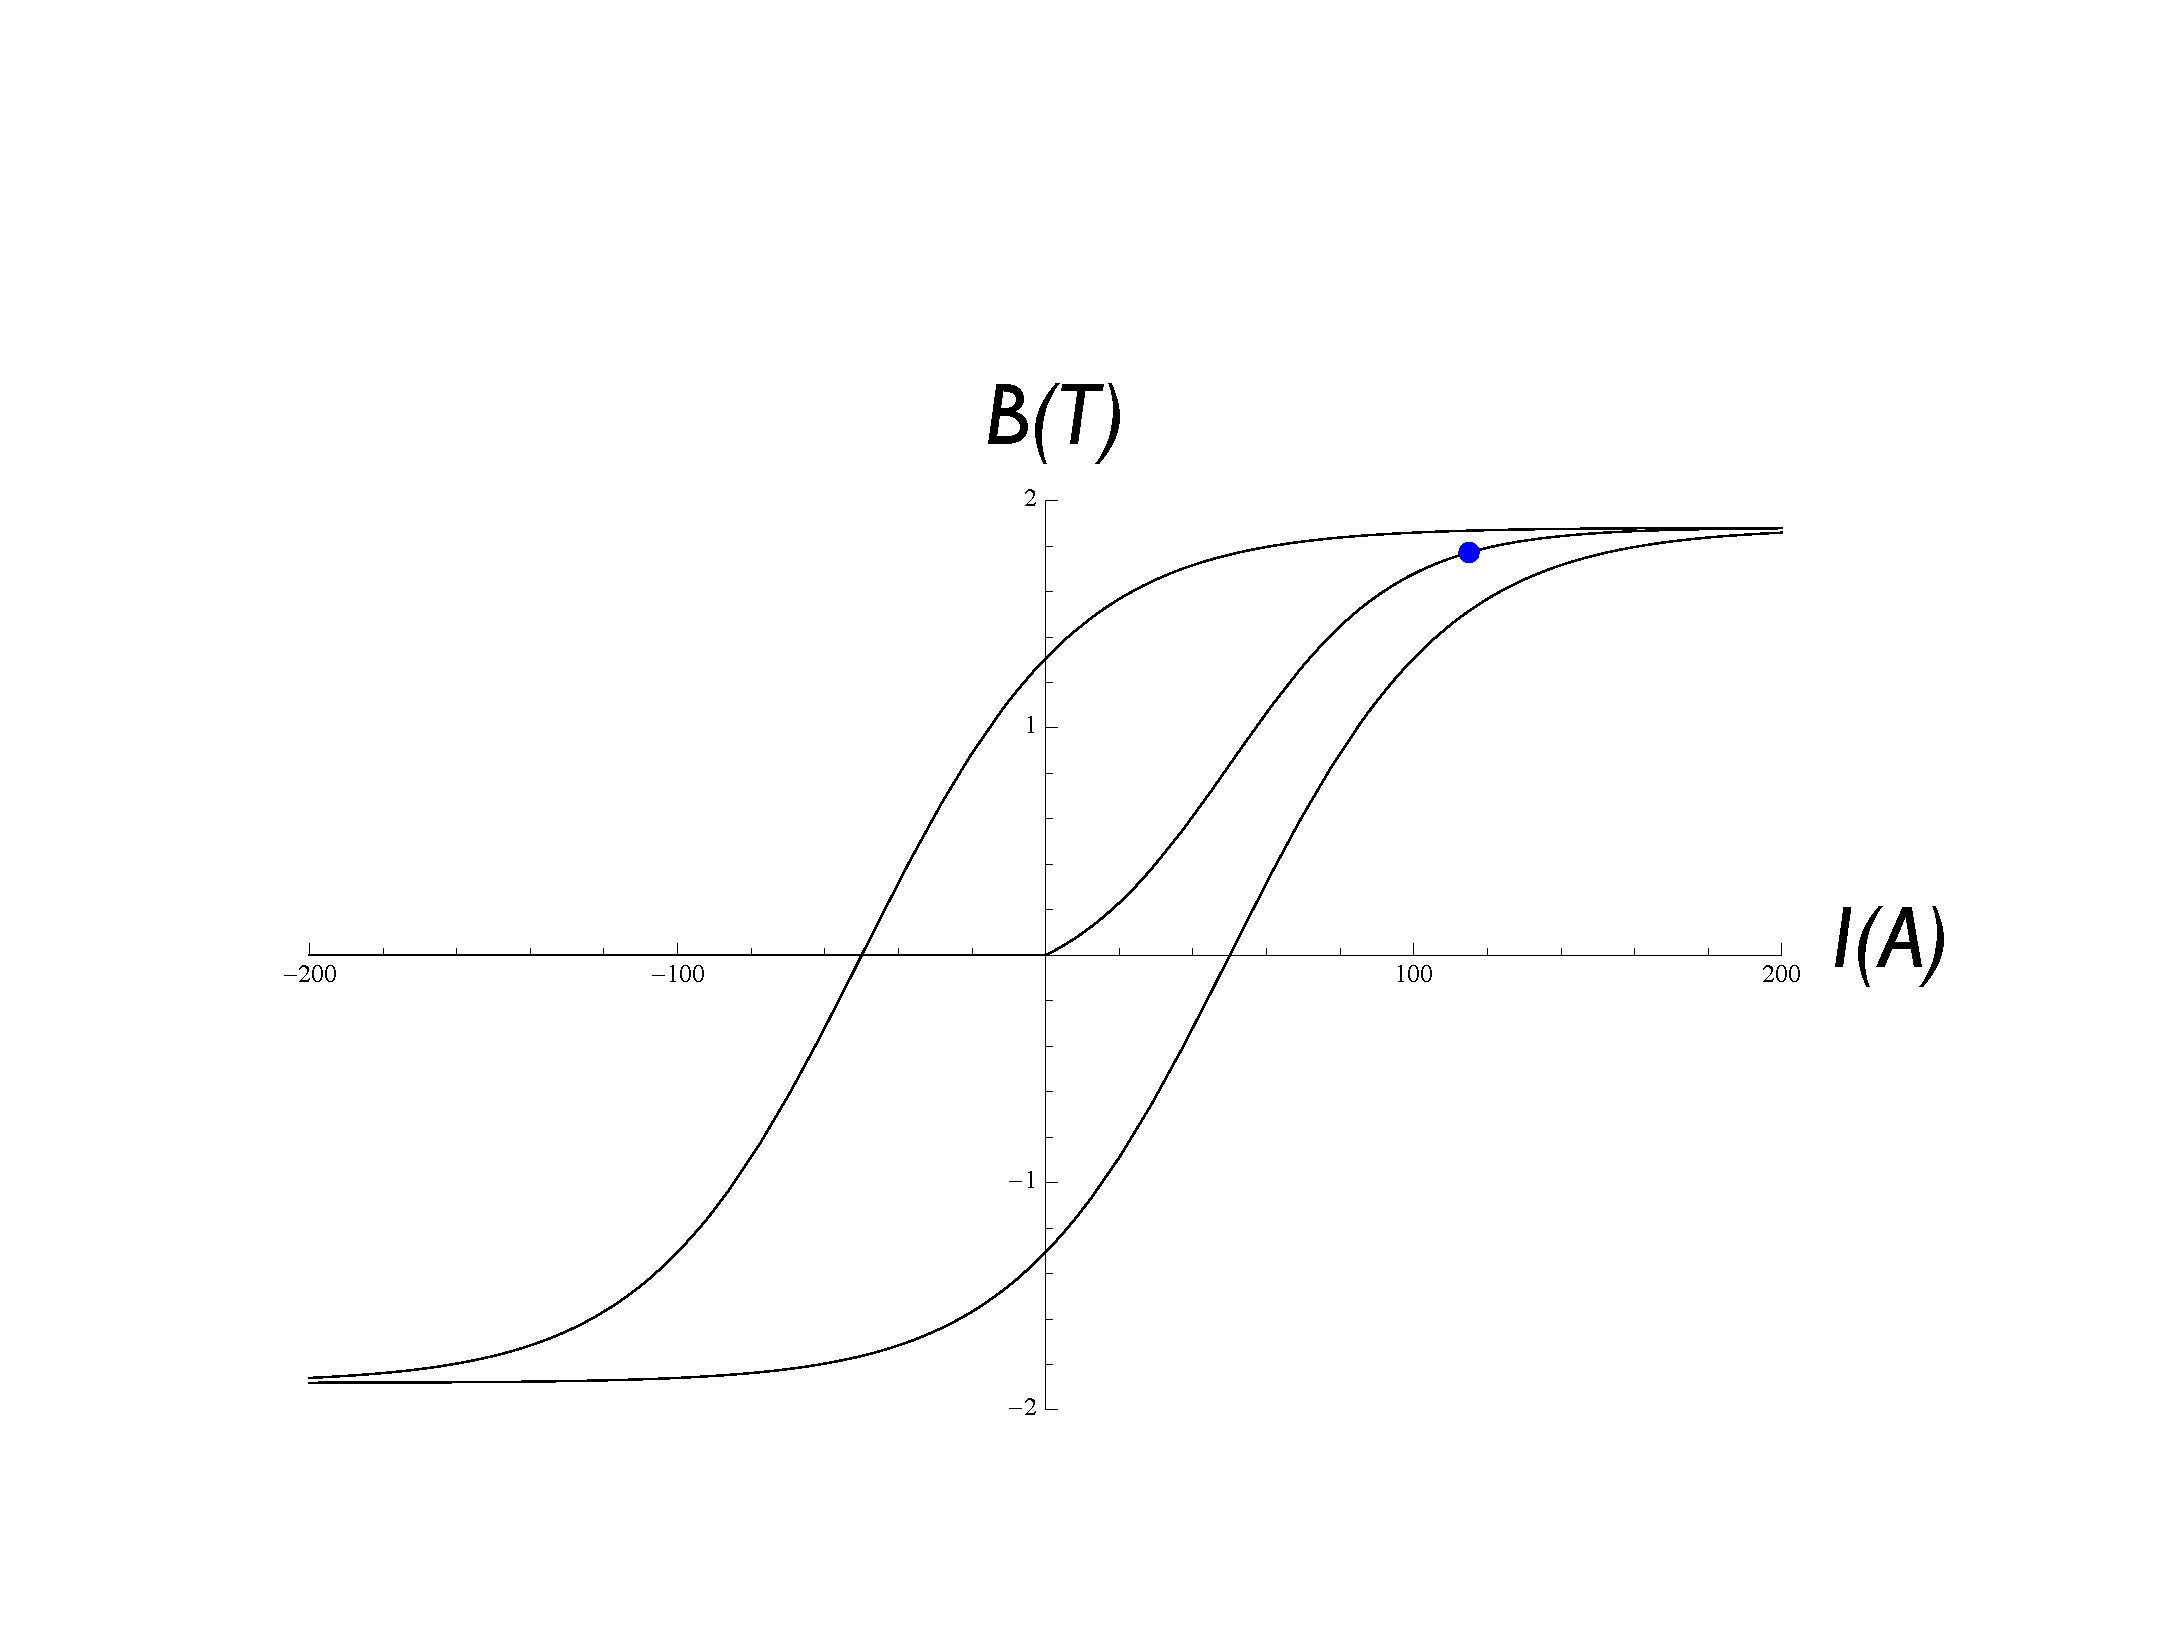
\includegraphics[width=0.6\textwidth]{figures/calib/tag/ecor/hysteresis_keynote.eps}
\caption[Plot Depicting the Process of Hysteresis]{\label{fig:hyst}Plot depicting the process of hysteresis. For the a current of strength I, there could exist two magnetic fields of strength B. Image source:~\cite{clas.thesis.kunkel}}
\end{center}\end{figure}

\FloatBarrier

Hysteresis would affect the scattered electron and was corrected for in the following manner. Lets let
\begin{align}
P_\text{π$^+$} + P_\text{π$^-$} = P_\text{π$^+$ π$^-$} \nonumber
\end{align}
therefore
\begin{align}
&(P_\text{γ} + P_\mathrm{target} - (P_\text{π$^+$π$^-$}))^2 = m_p^2 \\
& P_\text{γ}^2 + P_\mathrm{target}^2 + P_\text{π$^+$π$^-$}^2 + 2P_\text{γ}P_\mathrm{target} - 2P_\text{γ}P_\text{π$^+$π$^-$} - 2P_\mathrm{target}P_\text{π$^+$π$^-$}= m_p^2
\label{eq:tagger.energy}
\end{align}
collecting terms of $P_\text{γ}$ to one side and using $P_\mathrm{target}^2 = m_p^2 $ and $P_\text{γ}^2 = 0$
\begin{align}\label{eq:hyst.eqI}
 P_\text{π$^+$π$^-$}^2 - 2P_\mathrm{target}P_\text{π$^+$π$^-$}= 2P_\text{γ}(P_\text{π$^+$π$^-$} - P_\mathrm{target})
\end{align}
From this using eq.~\ref{eq:tagger.energy} in 4-vector notation
\begin{align}\label{eq:tagger.energyII}
P_\text{γ} = P_{E_0} - P_\text{e}\nonumber
\end{align}
where $P_{E_0}$ is the beam energy delivered from \abbr{CEBAF} as recorded in the \abbr{RUNC} bank and $P_\text{e}$ is the scattered electron in the \emph{bremsstrahlung} process that is recorded by the tagger. From eq.~\ref{eq:tagger.energy} the only known quantities are $P_{E_0}$ and $P_\text{γ}$. Applying a scalar correction to $P_\text{e}$ as $xP_\text{e}$ and solving for $x$ for all known quantities, eq.~\ref{eq:hyst.eqI} simplifies to;
\begin{align}
x= \frac{P_{E_0}(P_\mathrm{target}-P_\text{π$^+$π$^-$}) + P_\text{π$^+$π$^-$}^2/2  - P_\mathrm{target}P_\text{π$^+$π$^-$}}{(P_{E_0} - P_\text{γ})(P_\mathrm{target} - P_\text{π$^+$π$^-$})}
\end{align}
To reduce statistical fluctuations $\frac{1}{10}$ of run 56515 was analyzed to obtain the correction factor $x$. The correction factor was fitted to a $3^\mathrm{rd}$ order polynomial $\pm 0.008$ from the mean of the peak to establish an accurate measurement of the peak, this is shown in Fig.~\ref{fig:56515.cor}. After the correction factor was extracted for run 56515, it was applied to both the topologies listed in Eq.~\ref{eq:beam.cortopology} and Eq.~\ref{eq:beam.checktopology} by recalculating the photon beam energy as
\begin{align}
E_e = E_{\abbr{CEBAF}} - E_{γ} \nonumber \\
E_{γ}^{new} = E_{E_0} - E_e*x \nonumber.
\end{align}
Figures~\ref{fig:proton.fix} and \ref{fig:neutron.fix} illustrate the missing mass topologies after beam correction and shows that the new calculated missing mass is less than 1~MeV from \abbr{PDG} values. Since both the missing proton mass and missing neutron mass were adjusted properly to the correct mass by using the same beam correction factor, it shows that the correction factor is independent of topology and therefore must be applied to all \desg{g12} analyses. The procedure to calculate $x$ was repeated for every run in \desg{g12}, Fig.~\ref{fig:beamcor.run}, with $\frac{1}{10}$ of the data used. To validate the corrections of the entire \desg{g12} data set, the missing neutron mass was recalculated for each run, shown in  Fig.~\ref{fig:neutron.fixall}, using several correction schemes, i.e. a scheme of just ``energy-loss'' corrections, a scheme of ``energy-loss'' and momentum corrections (JTG PCor), a scheme of ``energy-loss'', momentum corrections (JTG PCor) and beam corrections (MK BeamCor) and a scheme of ``energy-loss'' and beam corrections (MK BeamCor). It can be seen in Fig.~\ref{fig:neutron.fixall} that the only scheme that sufficed was the combination of ``energy-loss'' and beam corrections.


\begin{figure}\begin{center}
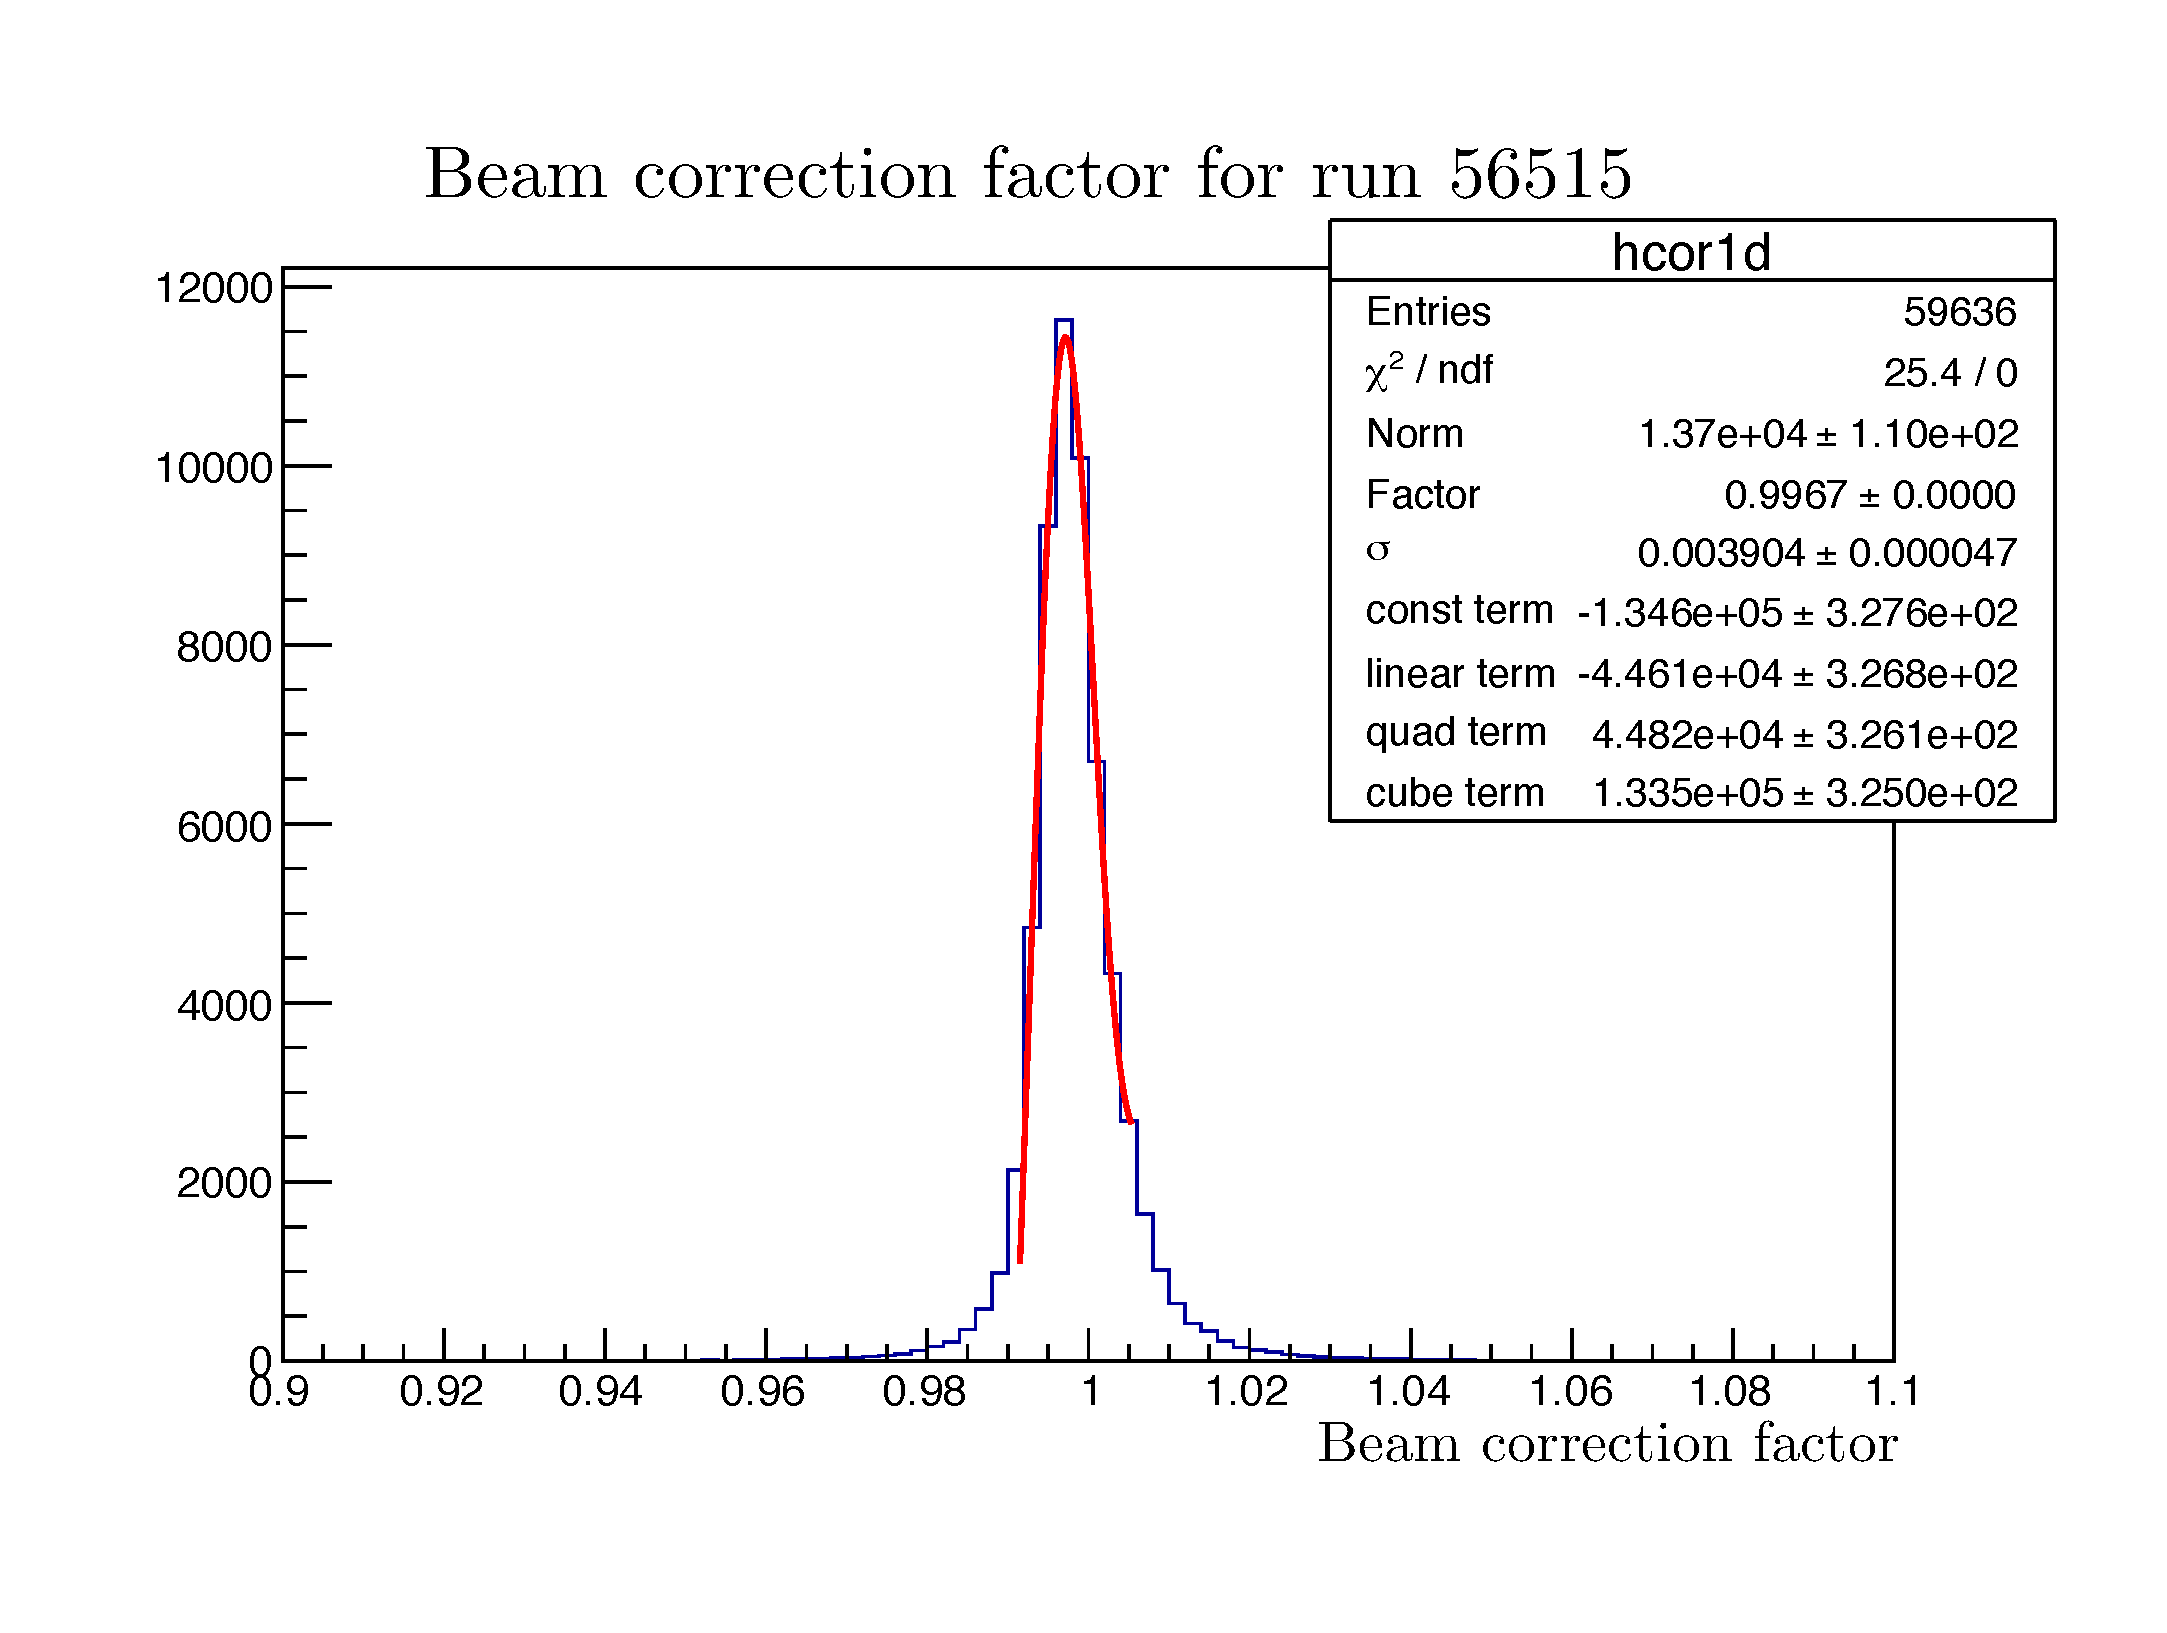
\includegraphics[width=0.6\textwidth]{figures/calib/tag/ecor/56515_cor.eps}
\caption[Beam Correction Factor for Run 56515]{\label{fig:56515.cor} Beam correction factor for run 56515. The fit is a $3^\mathrm{rd}$ order polynomial $\pm 0.008$ from the mean of the peak. Image source:~\cite{clas.thesis.kunkel}}
\end{center}\end{figure}

\begin{figure}\begin{center}
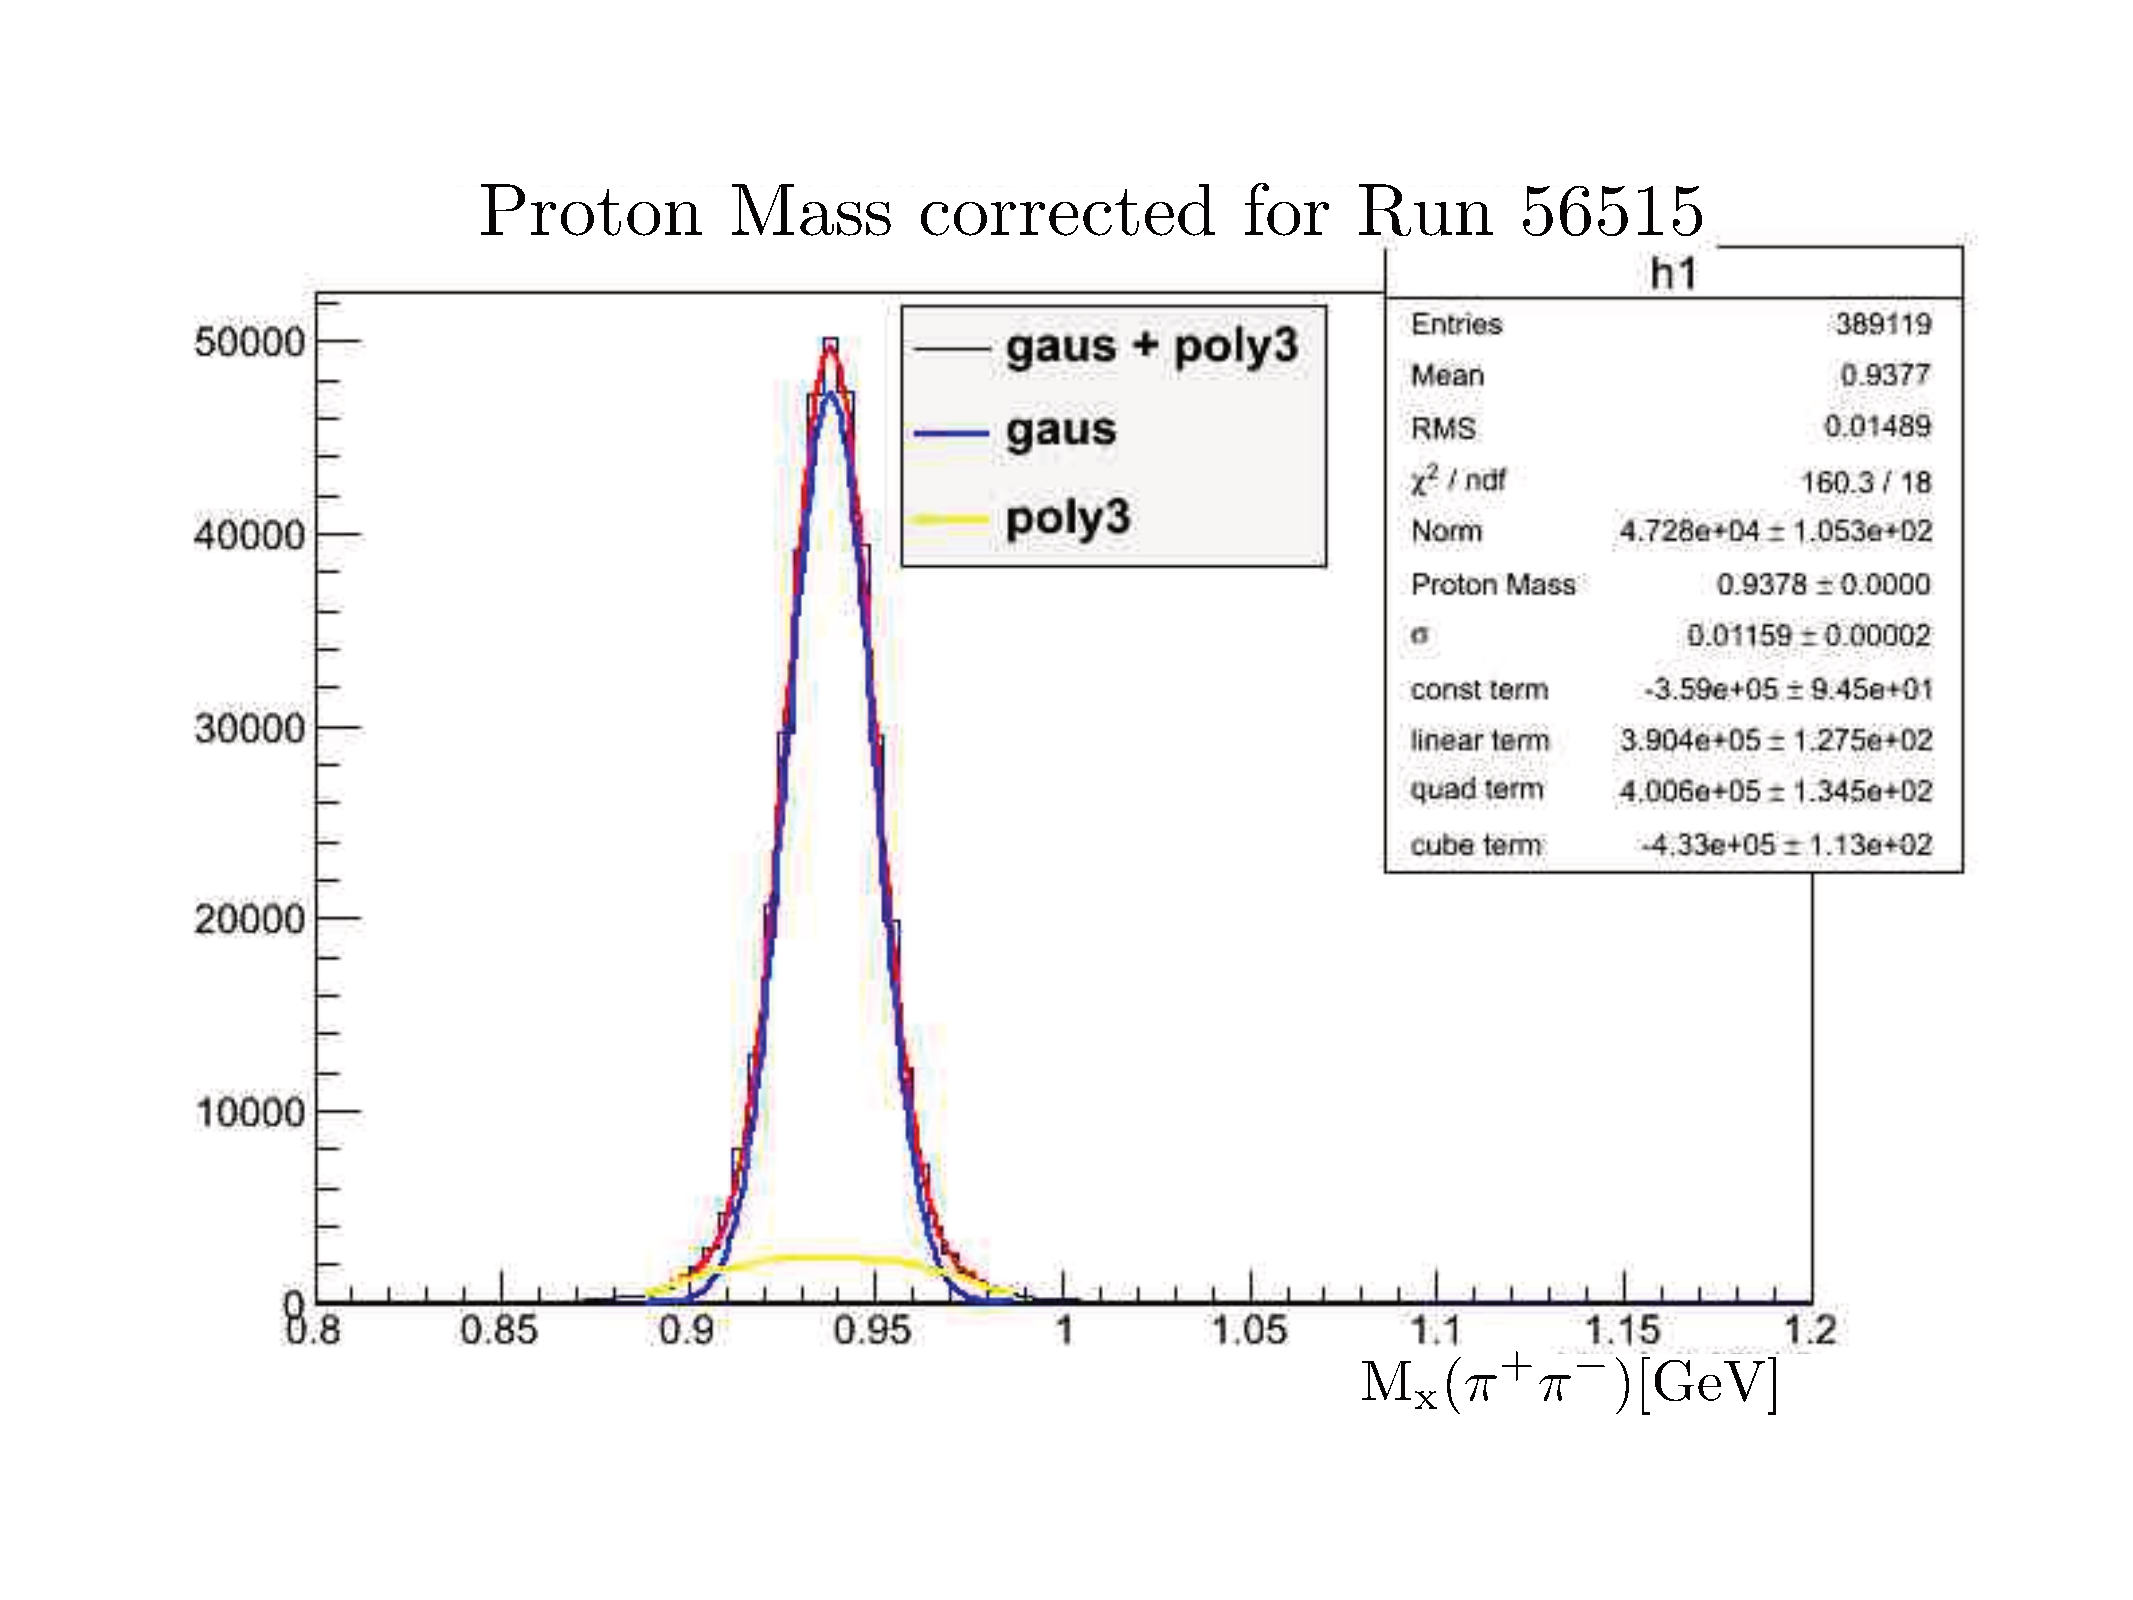
\includegraphics[width=0.6\textwidth]{figures/calib/tag/ecor/FixedmisssingmassII.pdf}
\caption[Proton Mass for Run 56515 After Beam Correction]{\label{fig:proton.fix} Plot of proton mass for runs 56515 after beam correction was applied.  \abbr{PDG} mass for the proton is 0.938272 GeV/c. Image source:~\cite{clas.thesis.kunkel}}
\end{center}\end{figure}

\begin{figure}\begin{center}
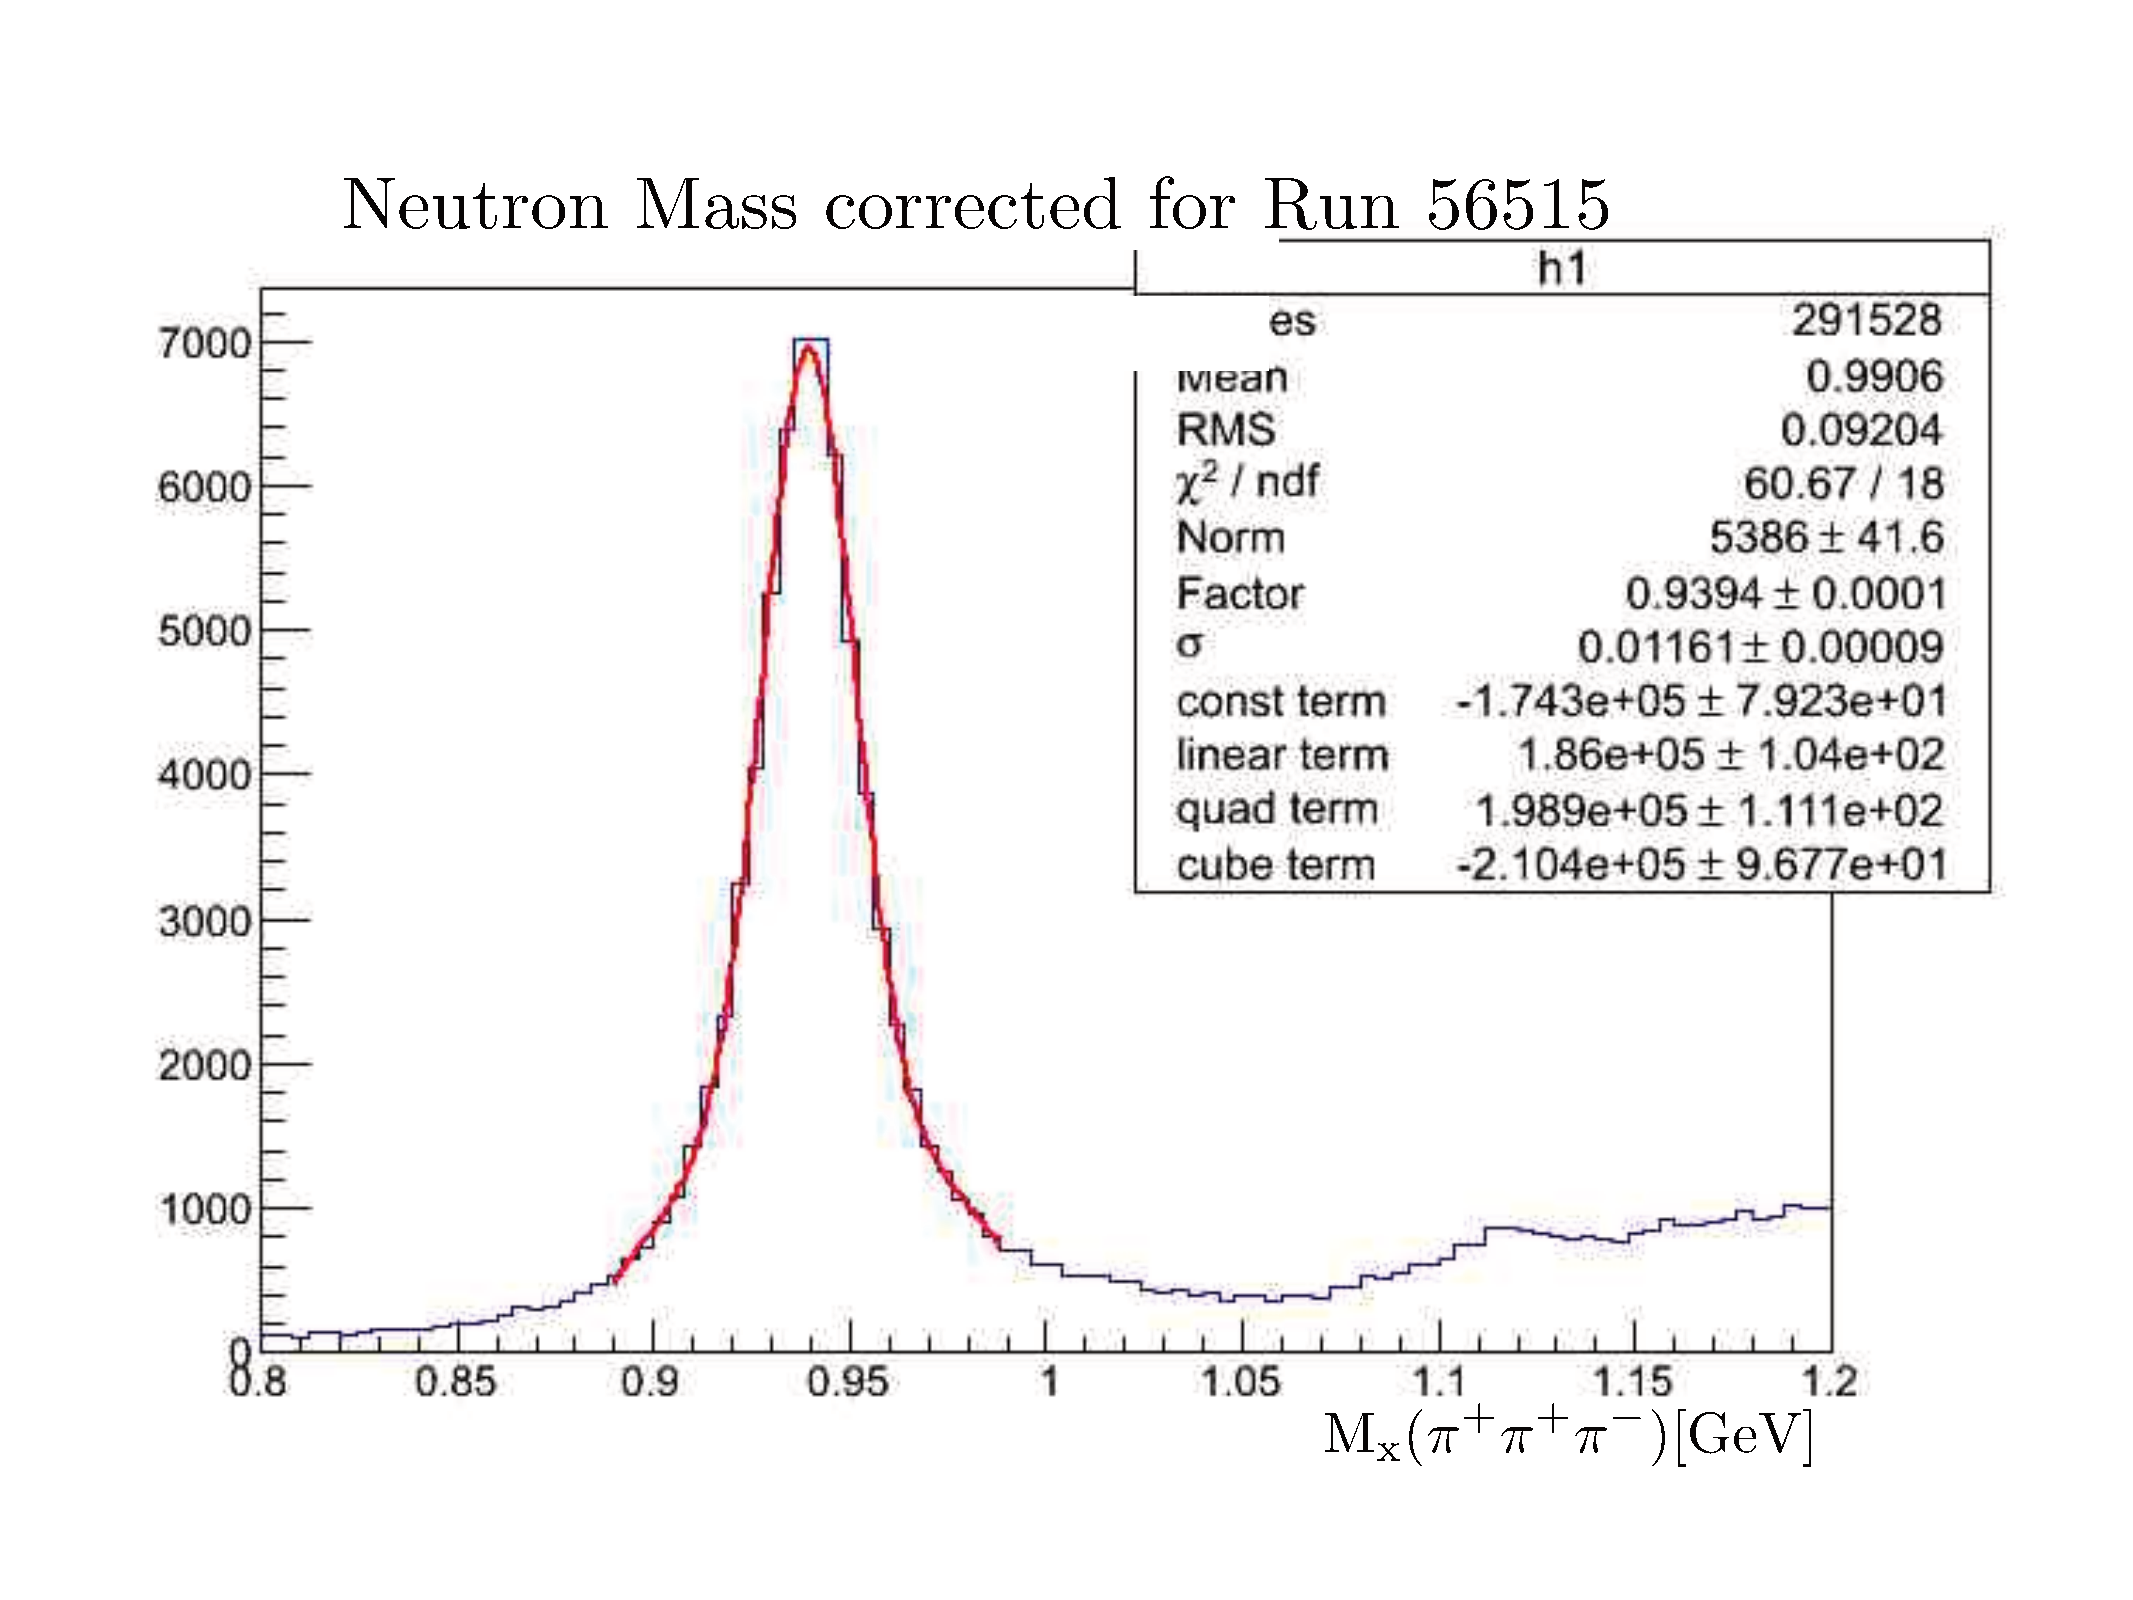
\includegraphics[width=0.6\textwidth]{figures/calib/tag/ecor/FixedmisssingmassneutronII.pdf}
\caption[Neutron Mass for Run 56515 After Beam Correction]{\label{fig:neutron.fix} Plot of neutron mass for runs 56515 after beam correction was applied  \abbr{PDG} mass for the neutron is 0.939565 GeV/c. In the plot, the "Factor" is the fitting parameter for the neutron mass. Image source:~\cite{clas.thesis.kunkel}}
\end{center}\end{figure}

\begin{figure}\begin{center}
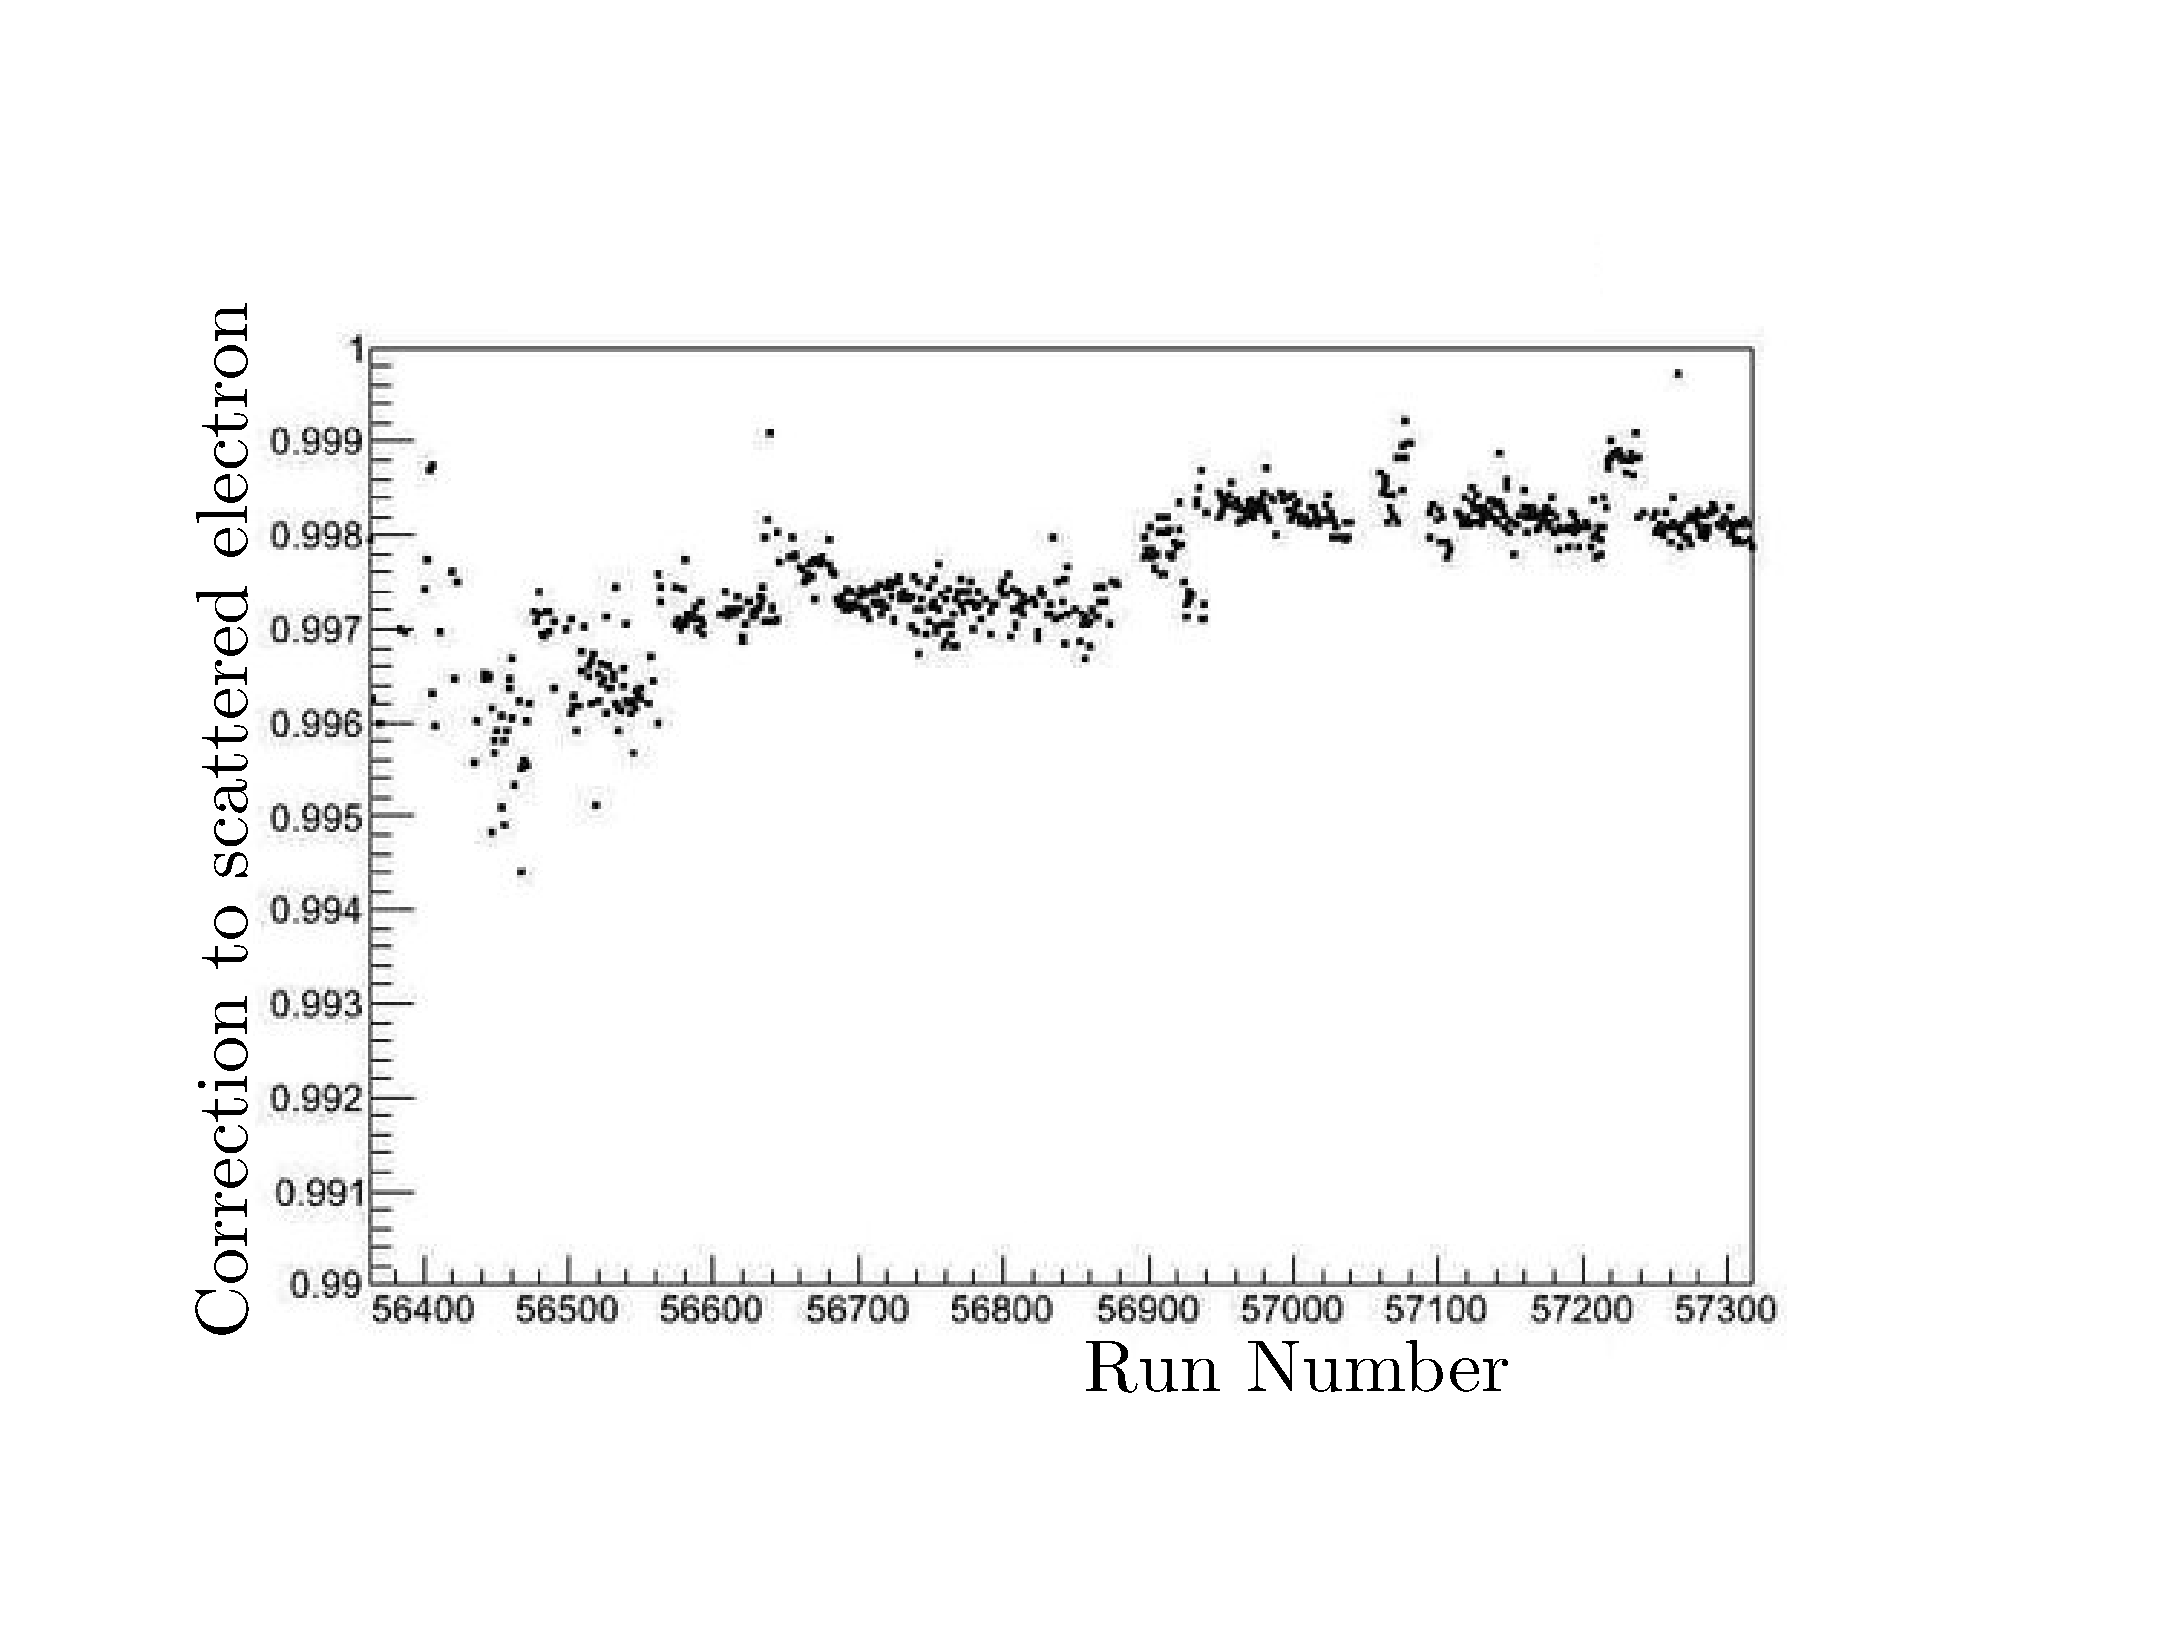
\includegraphics[width=0.6\textwidth]{figures/calib/tag/ecor/beam_cor.eps}
\caption[Beam Correction Factors for Entire \desg{g12} Runs]{\label{fig:beamcor.run} Plot of correction factor calculated for the entire \desg{g12} run set. Image source:~\cite{clas.thesis.kunkel}}
\end{center}\end{figure}

\begin{figure}\begin{center}
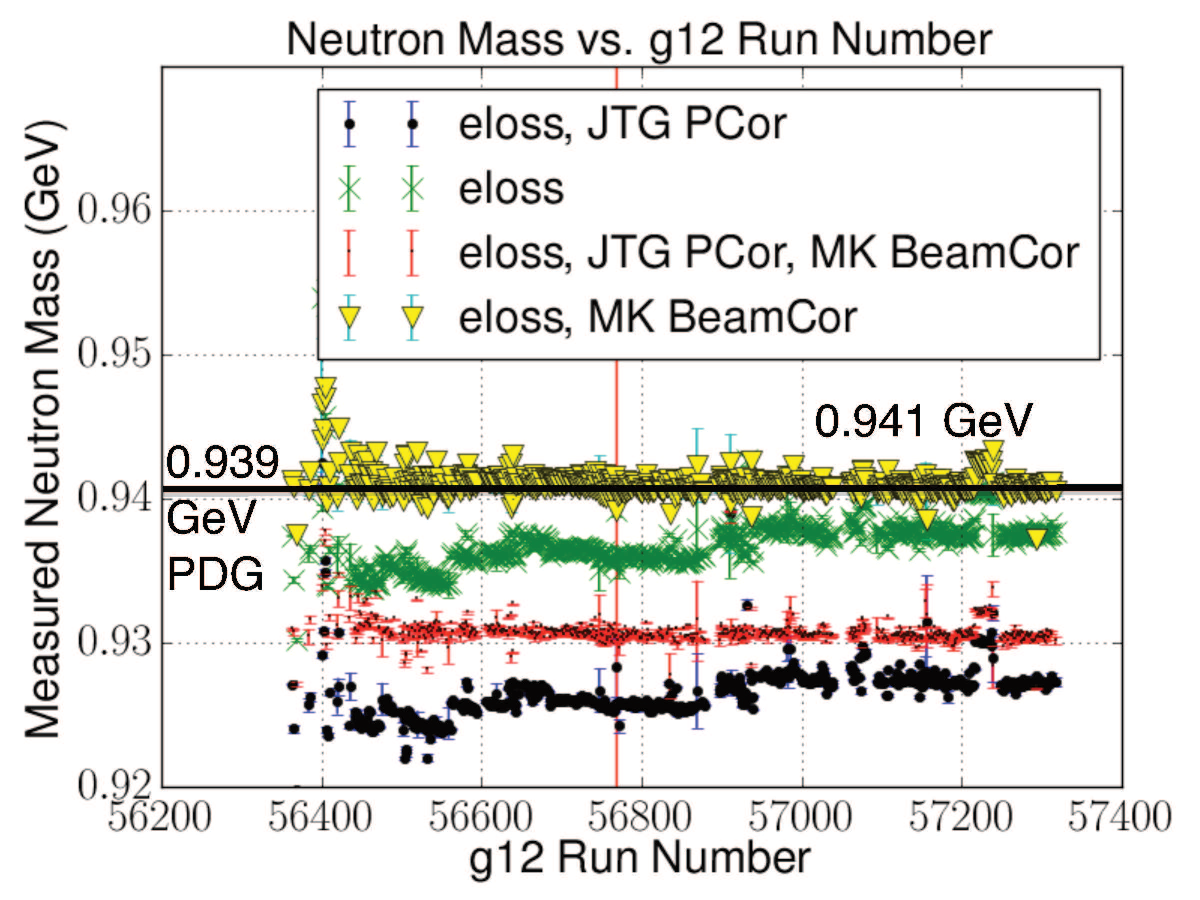
\includegraphics[width=0.6\textwidth]{figures/calib/tag/ecor/C3pi_allcorr_neutron_rxr.pdf}
\caption[Corrected Missing Neutron Mass for \desg{g12} Using Beam Corrections]{\label{fig:neutron.fixall} Plot of missing neutron mass using various corrections. The yellow triangles show a missing neutron mass with only ``energy-loss,'' beam corrections and momentum corrections applied. \abbr{PDG} mass for the neutron is 0.939565 GeV/c.}
\end{center}\end{figure}



To correct for run by run shifts in the beam energy, use the header file in:
\begin{verbatim}
g12_corrections.hpp
\end{verbatim}

In the analysis program, the user needs to have the run number of the event and the uncorrected beam energy, then use:
\begin{verbatim}
	Int_t run_input;
    if(run == 56400){run_input = 56401;}
    else if(run == 57314){run_input = 57315;}
    else{run_input = run;}
    egam_chosen_corrected = clas::g12::corrected_beam_energy(run_input, egam_chosen);
\end{verbatim}
The final and standard g12 photon-energy corrections were re-derived after the momentum correction and e-loss corrections were applied.
Here are some plots (Figs.~\ref{Test,TestII,TestIII,TestIV}) depicting the stability of the \Ks mass throughout the \pip and \pim momenta.

\begin{figure}\begin{center}
		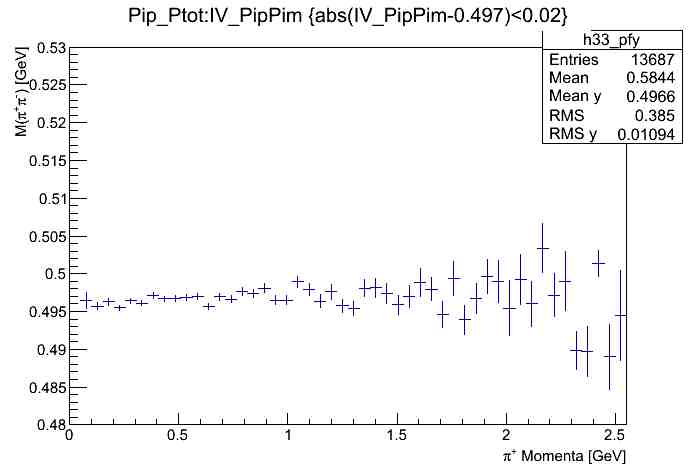
\includegraphics[width=0.6\textwidth]{MK_Response/MassvspIP.jpg}
		\caption[\Ks mass vs. \pip momentum.]{\label{fig:convprob_I} \Ks mass vs. \pip momentum.}
	\end{center}\end{figure}

\begin{figure}\begin{center}
		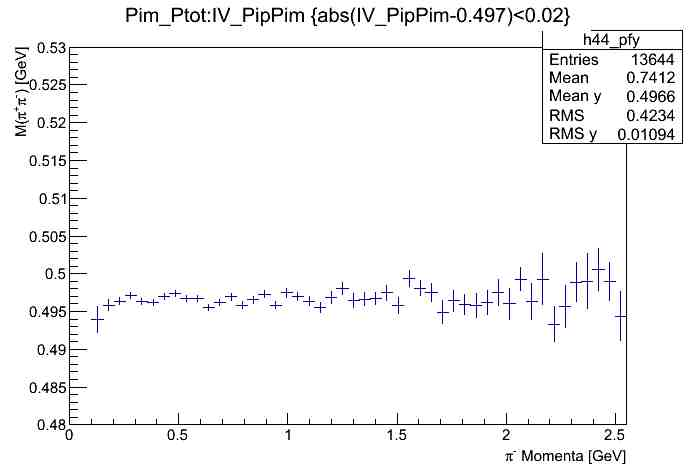
\includegraphics[width=0.6\textwidth]{MK_Response/Massvspim.jpg}
		\caption[\Ks mass vs. \pim momentum.]{\label{fig:convprob_II} \Ks mass vs. \pim momentum.}
	\end{center}\end{figure}
	Here are some plots (Figs.~\ref{fig:convprob_I,fig:convprob_II}) depicting the stability of the \Ks mass throughout the \pip and \pim the \pip and \pim polar angle $\theta$ and azimuthal angle $\phi$.
	
	\begin{figure}[h]
		\centering
			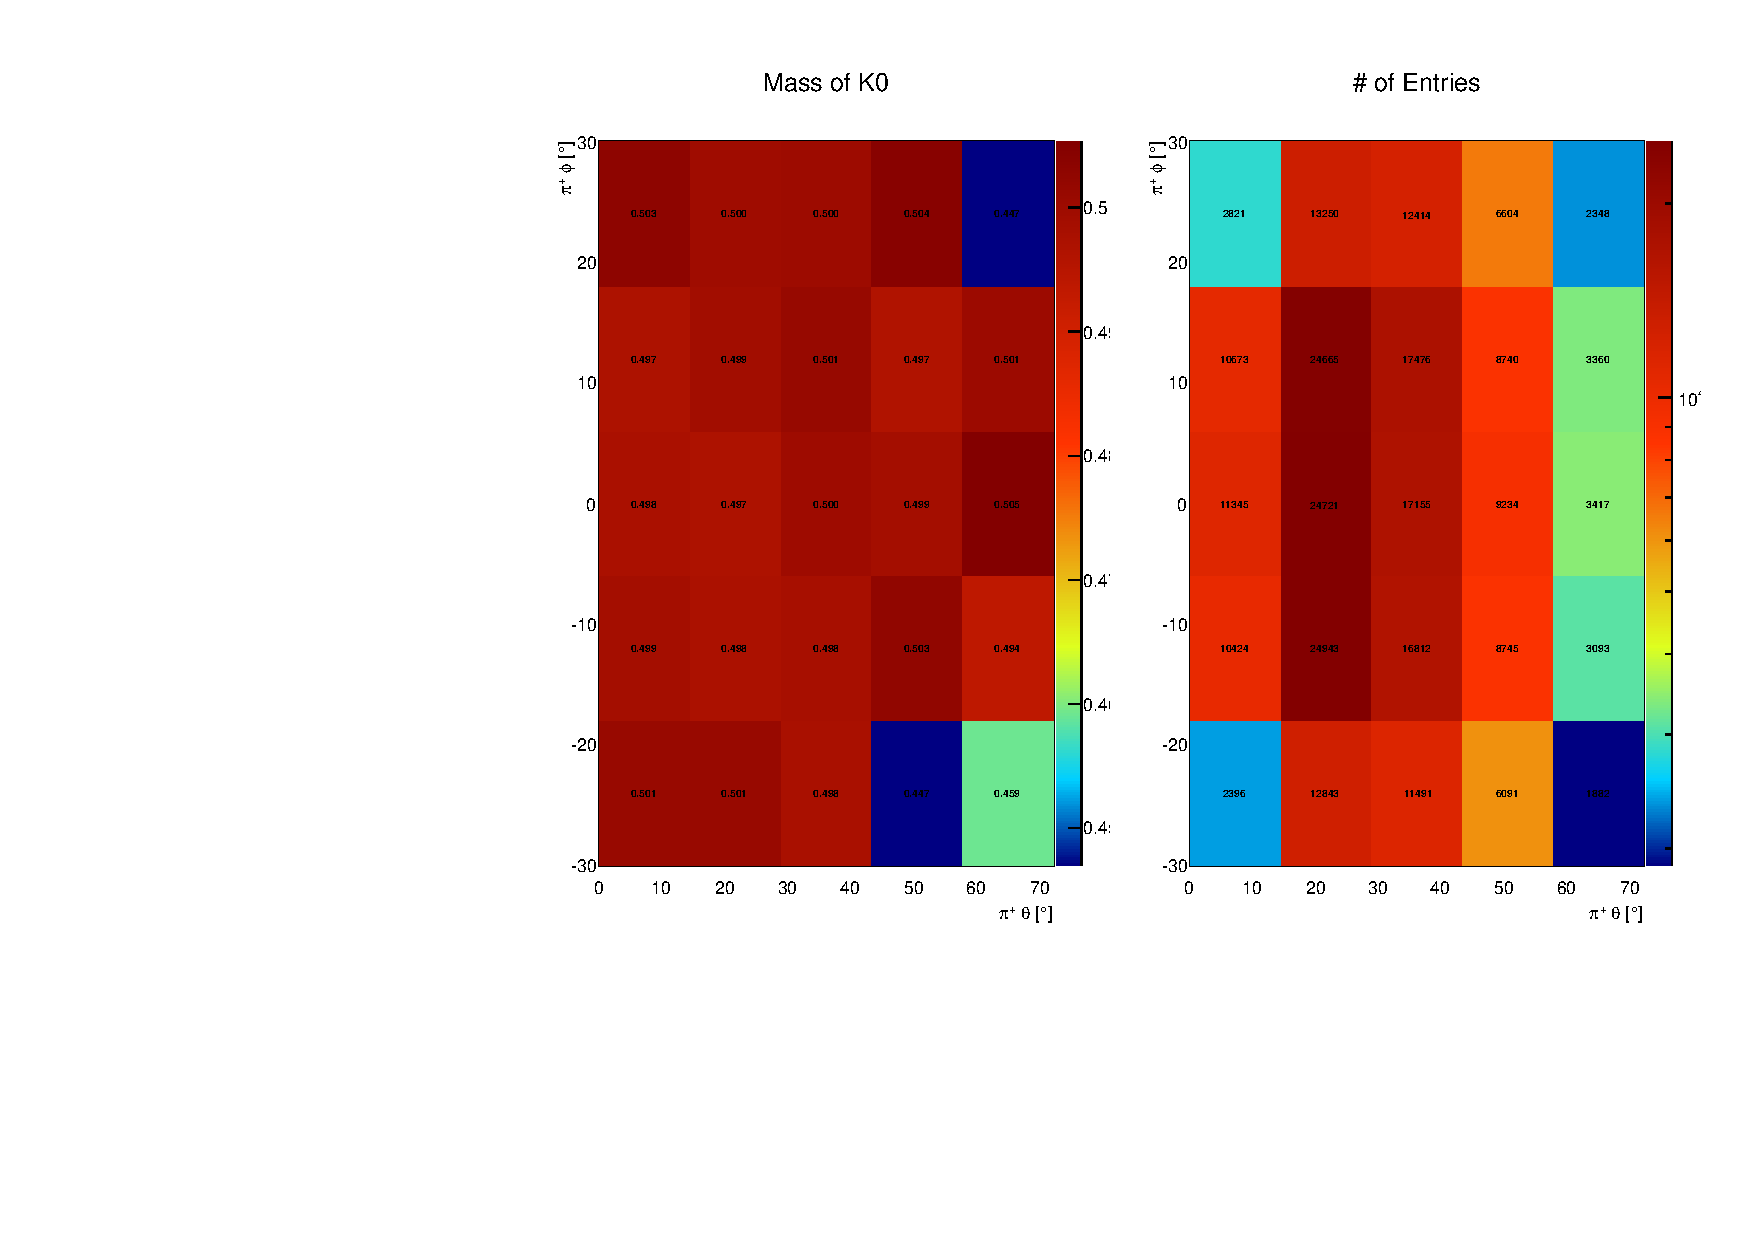
\includegraphics[page=1,width=.45\textwidth,rotate=-90]{MK_Response/PLOTS_FOR_56669/K0_OnePhi_C2.pdf} 
		\caption{(Left)\pip mod($\phi$) vs. $\theta$ with the centroid of the \Ks mass labeled. (Right)\pip mod($\phi$) vs. $\theta$ with the number of entries for the centroid of the \Ks mass labeled.}
		\label{fig:Test}
	\end{figure}
		\begin{figure}[h]
			\centering
				\includegraphics[page=2,width=.45\textwidth,rotate=-90]{MK_Response/PLOTS_FOR_56669/K0_OnePhi_C2.pdf} 
		\caption{(Left)\pim mod($\phi$) vs. $\theta$ with the centroid of the \Ks mass labeled. (Right)\pim mod($\phi$) vs. $\theta$ with the number of entries for the centroid of the \Ks mass labeled.}
			\label{fig:TestII}
		\end{figure}
	\begin{figure}[h]
		\centering
		\includegraphics[page=3,width=.45\textwidth,rotate=-90]{MK_Response/PLOTS_FOR_56669/K0_OnePhi_C2.pdf} 
		\caption{(Left)\pip mod($\phi$) vs. $\theta$ with the mass difference from PDG value of the \Ks mass labeled. (Right)\pip mod($\phi$) vs. $\theta$ with the number of entries for the mass difference of the \Ks mass labeled.}
		\label{fig:TestIII}
	\end{figure}
	\begin{figure}[h]
		\centering
		\includegraphics[page=4,width=.45\textwidth,rotate=-90]{MK_Response/PLOTS_FOR_56669/K0_OnePhi_C2.pdf} 
		\caption{(Left)\pim mod($\phi$) vs. $\theta$ with the mass difference from PDG value of the \Ks mass labeled. (Right)\pim mod($\phi$) vs. $\theta$ with the number of entries for the mass difference of the \Ks mass labeled.}
		\label{fig:TestIV}
	\end{figure}
 	 For some bins of $\theta$ and $\phi$ the \Ks mass difference (from PDG value) are more than 1 MeV, this is due to the number of entries and the fit performed for that bin. It should be noted that for all plots involving the $K_0$ mass distribution, a distance of closest approach cut was placed on the \pippim. 
 	 	 
\FloatBarrier
